\documentclass[10pt,xcolor={dvipsnames},fleqn]{beamer}
%\documentclass[handout,10pt,xcolor={dvipsnames},fleqn]{beamer}
\usepackage{isse}


\usepackage{apalike}
\usepackage[utf8]{inputenc}
\usepackage{pdfpages}
%\usepackage{ngerman}
\usepackage{stmaryrd,amsmath,amssymb}
\usepackage{color}
\usepackage{enumerate}
\usepackage[makeroom]{cancel}
\usepackage{mdframed}
\usepackage{xskak}
\usepackage{marvosym}
\setchessboard{
showmover=false}
\usepackage[noend]{algpseudocode}   % package for algorithms
\usepackage{algorithm}
\usepackage{tikz}

\usepackage[absolute,overlay]{textpos}

\usetikzlibrary{trees,calc,shapes,arrows,matrix,shadows,decorations.markings}
\usetikzlibrary{decorations.pathreplacing}

\mdfdefinestyle{theoremstyle}{
linecolor=red,linewidth=2pt,
frametitlerule=true,
frametitlebackgroundcolor=gray!20,
innertopmargin=\topskip,
}
\definecolor{LRed}{rgb}{1,.8,.8}
\definecolor{MRed}{rgb}{1,.6,.6}
\definecolor{HRed}{rgb}{1,.2,.2}

\usepackage{listings}
\lstdefinelanguage{mzn}
{
	morekeywords={var,int,solve,not,search,satisfy,endif,maximize,minimize,float,constraint,sum,forall,exists,array,of,include,predicate,then,commit,post,set,function,if,else,repeat,next,ann,break},
	sensitive=false,
	morecomment=[l]{\%},
	morecomment=[s]{/*}{*/},
	morestring=[b]",
}

\definecolor{lightlightgray}{gray}{0.95}
\definecolor{forestgreen}{HTML}{009B55}
\definecolor{thermicred}{rgb}{0.82, 0.1, 0.26}
\lstset
{
	basicstyle=\ttfamily\small,
	commentstyle=\ttfamily\color{thermicred},
	stringstyle=\ttfamily\color{isseorange},
	keywordstyle=\ttfamily\color{blue},
	tabsize=2,
	showstringspaces=false,
	flexiblecolumns=true,
	captionpos=b,	
	backgroundcolor=\color{lightlightgray},
	frame=single,
	 xleftmargin=\parindent,
}

\lstset{language=mzn}
\interfootnotelinepenalty=10000

% ====== custom commands

\newcommand{\prosumer}[1]{\ensuremath{\mathtt{#1}}}
% Soft Constraint Example
\newcommand{\constraintName}[1]{\ensuremath{\mathtt{#1}}}
% Biogas Constraints
\newcommand{\biogas}{biogas}
\newcommand{\biogasShort}{bio}
\newcommand{\gasFull}{\ensuremath{\constraintName{gasFull}_\mathtt{\biogasShort}}}
\newcommand{\ecoSweet}{\ensuremath{\constraintName{ecoSweet}_\mathtt{\biogasShort}}}
\newcommand{\onOff}{\ensuremath{\constraintName{onOff}_\mathtt{\biogasShort}}}
% Thermal Plant Constraints
\newcommand{\thermal}{thermal}
\newcommand{\thermalShort}{therm}
\newcommand{\ecoOpt}{\ensuremath{\constraintName{ecoOpt}_\mathtt{\thermalShort}}}
\newcommand{\inertia}{\ensuremath{\constraintName{inertia}_\mathtt{\thermalShort}}}
\newcommand{\ecoGood}{\ensuremath{\constraintName{ecoGood}_\mathtt{\thermalShort}}}
\newcommand{\hLevelThermal}[1]{$H_#1^\mathtt{\thermalShort}$}
% Electric Vehicle
\newcommand{\ev}{EV}
\newcommand{\limitBatteryUsage}{\ensuremath{\constraintName{limitBU}_\mathtt{\ev}}}
\newcommand{\prefBatteryLevel}{\ensuremath{\constraintName{prefBL}_\mathtt{\ev}}}
\newcommand{\earlyBird}{\ensuremath{\constraintName{earlyBird}_\mathtt{\ev}}}
% Organization
\newcommand{\org}{org}
\newcommand{\minMaxViolation}{\ensuremath{\constraintName{violation}_\mathtt{\org}}}
\newcommand{\hLevelOrg}[1]{$H_#1^\mathtt{\org}$}

\newcommand{\Variable}{X}
\newcommand{\LocalVariable}{\widehat{\Variable}}
\newcommand{\Domain}{D}
\newcommand{\Constraint}{C}
\newcommand{\ConstraintRelationship}{\mathcal{R}}

\newcommand{\valuation}{v}
\newcommand{\constraint}[1]{\mathrm{#1}}

\newcommand{\plantconstraint}[3]{  
\ifx#1b \constraint{best}[#3]
\else \ifx#1g \constraint{good}[#3]
\else \ifx#1a \constraint{acc}[#3]
\else \ifx#1d \constraint{diff}
\else \ifx#1l \constraint{low}[#3]
\else \ifx#1h \constraint{high}[#3]
\else \ifx#1o \constraint{org}[#3]
   \else
   \constraint{#1}_{#2}^{#3} 
   
   
\fi \fi \fi \fi \fi \fi \fi}
\usepackage{stmaryrd}

\newcommand{\code}[1]{\normalfont\texttt{\spaceskip=3pt\frenchspacing\def\{{\char123}\def\}{\char125}\def\^{\char94}\def\_{\char95}#1}}
\newcommand{\varit}[1]{{\frenchspacing\ensuremath{\normalfont\textsl{#1}}}}
\newcommand{\macit}[1]{{\frenchspacing\ensuremath{\normalfont\textsf{#1}}}}
\newcommand{\Eta}{\mathrm{H}}
\newcommand{\Mu}{\mathrm{M}}
\newcommand{\Nu}{\mathrm{N}}

\newcommand{\NZ}{\mathbb{N}}
\newcommand{\RZ}{\mathbb{R}}
\newcommand{\RZp}{\RZ_{\geq 0}}
\newcommand{\powerset}{\mathcal{P}}
\newcommand{\limp}{\mathrel{\Rightarrow}}
\newcommand{\compfun}{\mathbin{\circ}}
\newcommand{\isorel}{\mathrel{\cong}}
\newcommand{\restrict}[2]{{#1}\mathnormal{\upharpoonright}{#2}}
\newcommand{\natto}{\mathrel{\dot{\mathnormal{\to}}}}
\let\lbagold\lbag
\let\rbagold\rbag
\def\lbag{\mathopen{\lbagold}}
\def\rbag{\mathclose{\rbagold}}

\DeclareMathOperator{\Minop}{\mathrm{Min}}
\newcommand{\Min}[1]{\Minop^{#1}}
\DeclareMathOperator{\Maxop}{\mathrm{Max}}
\newcommand{\Max}[1]{\Maxop^{#1}}
\DeclareMathOperator{\finsets}{\mathcal{P}_{\mathrm{fin}}}
\DeclareMathOperator{\nefinsets}{\mathcal{P}_{\mathrm{fin}^+}}
%\DeclareMathOperator{\incfinsets}{\mathcal{I}_{\mathrm{fin}}}
\newcommand{\incfinsets}[1]{\mathcal{I}_{\mathrm{fin}}^{#1}}
\newcommand{\lowersubseteq}[1]{\mathrel{\subseteq_{#1}}}
\newcommand{\lowersupseteq}[1]{\mathrel{\supseteq_{#1}}}
\newcommand{\lowersubset}[1]{\mathrel{\subset_{#1}}}
\newcommand{\lowersupset}[1]{\mathrel{\supset_{#1}}}
\newcommand{\uppersubseteq}[1]{\mathrel{\subseteq^{#1}}}
\newcommand{\uppersupseteq}[1]{\mathrel{\supseteq^{#1}}}
\newcommand{\uppersubset}[1]{\mathrel{\subset^{#1}}}
\newcommand{\uppersupset}[1]{\mathrel{\supset^{#1}}}
\newcommand{\lowercup}[1]{\mathbin{\cup_{#1}}}
\newcommand{\uppercup}[1]{\mathbin{\cup^{#1}}}

\DeclareMathOperator{\finmsets}{\mathcal{M}_{\mathrm{fin}}}
\DeclareMathOperator{\nefinmsets}{\mathcal{M}_{\mathrm{fin}^+}}
\newcommand{\mcup}{\mathbin{\mathnormal{\cup}\llap{\text{\fontsize{8pt}{8pt}\selectfont$-$}}}}
\newcommand{\submseteq}{%
\mathrel{\mathchoice%
{\mathnormal{\subseteq}\llap{\text{\raisebox{0.3pt}{\fontsize{8pt}{8pt}\selectfont\rotatebox{90}{$-$}\hspace{1.8pt}}}}}%
{\mathnormal{\subseteq}\llap{\text{\raisebox{0.3pt}{\fontsize{8pt}{8pt}\selectfont\rotatebox{90}{$-$}\hspace{1.8pt}}}}}%
{\mathnormal{\subseteq}\llap{\text{\raisebox{-0.3pt}{\fontsize{5pt}{5pt}\selectfont\rotatebox{90}{$-$}\hspace{1.4pt}}}}}%
{\mathnormal{\subseteq}\llap{\text{\raisebox{-0.3pt}{\fontsize{5pt}{5pt}\selectfont\rotatebox{90}{$-$}\hspace{1.4pt}}}}}%
}}
\newcommand{\supmseteq}{\mathrel{\reflectbox{$\submseteq$}}}
\newcommand{\lowersubmseteq}[1]{\mathrel{\submseteq_{#1}}}
\newcommand{\uppersubmseteq}[1]{\mathrel{\submseteq^{#1}}}
\newcommand{\submset}{%
\mathrel{\mathchoice%
{\mathnormal{\subset}\llap{\text{\raisebox{-0.8pt}{\fontsize{8pt}{8pt}\selectfont\rotatebox{90}{$-$}\hspace{1.8pt}}}}}%
{\mathnormal{\subset}\llap{\text{\raisebox{-0.8pt}{\fontsize{8pt}{8pt}\selectfont\rotatebox{90}{$-$}\hspace{1.8pt}}}}}%
{\mathnormal{\subset}\llap{\text{\raisebox{-0.3pt}{\fontsize{7pt}{7pt}\selectfont\rotatebox{90}{$-$}\hspace{1pt}}}}}%
{\mathnormal{\subset}\llap{\text{\raisebox{-0.3pt}{\fontsize{7pt}{7pt}\selectfont\rotatebox{90}{$-$}\hspace{1pt}}}}}%
}}
\newcommand{\supmset}{\mathrel{\reflectbox{$\submset$}}}
\newcommand{\lowersubmset}[1]{\mathrel{\submset_{#1}}}
\newcommand{\uppersubmset}[1]{\mathrel{\submset^{#1}}}

\DeclareMathOperator{\collapseset}{\mathcal{C}}

\newcommand{\category}[1]{\mathrm{#1}}
\newcommand{\POcat}{\category{PO}}
\newcommand{\uSLcat}{\category{uSL}}
\newcommand{\poMoncat}{\category{poMon}}
\newcommand{\jMoncat}{\category{jMon}}
\newcommand{\mMoncat}{\category{mMon}}
\newcommand{\xMoncat}{{x}\category{Mon}}
\newcommand{\PVScat}{\category{PVS}}
\newcommand{\cSRngcat}{\category{cSRng}}
\newcommand{\DAGcat}{\category{DAG}}

\newcommand{\idfun}[1]{1_{#1}}
\newcommand{\functor}[1]{\mathit{#1}}
\DeclareMathOperator{\POfun}{\functor{PO}}
\DeclareMathOperator{\uSLfun}{\functor{uSL}}
\DeclareMathOperator{\poMonfun}{\functor{poMon}}
\DeclareMathOperator{\jMonfun}{\functor{jMon}}
\DeclareMathOperator{\mMonfun}{\functor{mMon}}
\DeclareMathOperator{\xMonfun}{\text{$x$}\functor{Mon}}
\DeclareMathOperator{\PVSfun}{\functor{PVS}}
\DeclareMathOperator{\cSRngfun}{\functor{cSRng}}
\DeclareMathOperator{\DAGfun}{\functor{DAG}}

\newcommand{\uSLfree}[1]{\uSLfun\langle#1\rangle}
\newcommand{\uSLeta}{\eta^{\uSLcat}}
\newcommand{\uSLetaat}[1]{\uSLeta_{#1}}
\newcommand{\uSLlift}[1]{{#1}^{\sharp_{\uSLcat}}}

\newcommand{\poMonfree}[1]{\poMonfun\langle#1\rangle}
\newcommand{\poMoneta}{\eta^{\poMoncat}}
\newcommand{\poMonetaat}[1]{\poMoneta_{#1}}
\newcommand{\poMonlift}[1]{{#1}^{\sharp_{\poMoncat}}}

\newcommand{\jMonfree}[1]{\jMonfun\langle#1\rangle}
\newcommand{\jMoneta}{\eta^{\jMoncat}}
\newcommand{\jMonetaat}[1]{\jMoneta_{#1}}
\newcommand{\jMonlift}[1]{{#1}^{\sharp_{\jMoncat}}}

\newcommand{\mMonfree}[1]{\mMonfun\langle#1\rangle}
\newcommand{\mMoneta}{\eta^{\mMoncat}}
\newcommand{\mMonetaat}[1]{\mMoneta_{#1}}
\newcommand{\mMonlift}[1]{{#1}^{\sharp_{\mMoncat}}}

\newcommand{\PVSfree}[1]{\PVSfun\langle#1\rangle}
\newcommand{\PVSeta}{\eta^{\PVScat}}
\newcommand{\PVSetaat}[1]{\PVSeta_{#1}}
\newcommand{\PVSlift}[1]{{#1}^{\sharp_{\PVScat}}}

\newcommand{\xMonfree}[1]{\xMonfun\langle#1\rangle}
\newcommand{\xMoneta}{\eta^{\xMoncat}}
\newcommand{\xMonetaat}[1]{\xMoneta_{#1}}
\newcommand{\xMonlift}[1]{{#1}^{\sharp_{\xMoncat}}}

\newcommand{\cSRngfree}[1]{\cSRngfun\langle#1\rangle}
\newcommand{\cSRngeta}{\eta^{\cSRngcat}}
\newcommand{\cSRngetaat}[1]{\cSRngeta_{#1}}
\newcommand{\cSRnglift}[1]{{#1}^{\sharp_{\cSRngcat}}}

\newcommand{\POfree}[1]{\POfun\langle#1\rangle}
\newcommand{\POeta}{\eta^{\POcat}}
\newcommand{\POetaat}[1]{\POeta_{#1}}
\newcommand{\POlift}[1]{{#1}^{\sharp_{\POcat}}}

\newcommand{\mtimes}[1]{\mathbin{\tilde{\cdot}_{#1}}}
\newcommand{\mplus}[1]{\mathbin{\tilde{\cup}_{#1}}}
\newcommand{\ftimes}[1]{\mathbin{\tilde{\mcup}^{#1}}}
\newcommand{\fplus}[1]{\mathbin{\tilde{\cup}_{#1}}}

\DeclareMathOperator{\scope}{\mathrm{sc}}
\DeclareMathOperator{\defdom}{\mathrm{def}}

\newcommand{\reflclos}[1]{\mathrel{(#1)^=}}
\newcommand{\transclos}[2][+]{\mathrel{(#2)^{#1}}}
\newcommand{\refltransclos}[1]{\mathrel{(#1)^*}}

\newcommand{\XPDrel}[2][\pi]{\rightsquigarrow^{#1}_{#2}}
\newcommand{\XPDreleq}[2][\pi]{\rightsquigarrow^{#1, =}_{#2}}
\newcommand{\XPDord}[2][\pi]{<^{#1}_{#2}}
\newcommand{\XPDordeq}[2][\pi]{\geq^{#1}_{#2}}
\newcommand{\XPDleq}[2][\pi]{\leq^{#1}_{#2}}
\newcommand{\XPDgeq}[2][\pi]{\geq^{#1}_{#2}}
\newcommand{\XPDw}[2][\pi]{w^{#1}_{#2}}
\newcommand{\XPDW}[2][\pi]{W^{#1}_{#2}}
\newcommand{\XPDk}[2][\pi]{k^{#1}_{#2}}

\newcommand{\SPDrel}{\XPDrel[\mathrm{SPD}]}
\newcommand{\SPDreleq}{\XPDreleq[\mathrm{SPD}]}
\newcommand{\SPDleq}{\XPDleq[\mathrm{SPD}]}
\newcommand{\SPDgeq}{\XPDgeq[\mathrm{SPD}]}
\newcommand{\SPDord}{\XPDord[\mathrm{SPD}]}
\newcommand{\SPDw}{\XPDw[\mathrm{SPD}]}
\newcommand{\SPDW}{\XPDW[\mathrm{SPD}]}
\newcommand{\DPDrel}{\XPDrel[\mathrm{DPD}]}
\newcommand{\DPDreleq}{\XPDreleq[\mathrm{DPD}]}
\newcommand{\DPDord}{\XPDord[\mathrm{DPD}]}
\newcommand{\DPDw}{\XPDw[\mathrm{DPD}]}
\newcommand{\DPDW}{\XPDW[\mathrm{DPD}]}
\newcommand{\TPDrel}{\XPDrel[\mathrm{TPD}]}
\newcommand{\TPDreleq}{\XPDreleq[\mathrm{TPD}]}
\newcommand{\TPDleq}{\XPDleq[\mathrm{TPD}]}
\newcommand{\TPDgeq}{\XPDgeq[\mathrm{TPD}]}
\newcommand{\TPDord}{\XPDord[\mathrm{TPD}]}
\newcommand{\TPDw}{\XPDw[\mathrm{TPD}]}
\newcommand{\TPDW}{\XPDW[\mathrm{TPD}]}

\DeclareMathSymbol{\UPi}{\mathalpha}{operators}{"05}



\renewcommand{\submseteq}{%
\mathrel{\mathchoice%
{\mathnormal{\subseteq}\llap{\text{\raisebox{0.0pt}{\fontsize{7.5pt}{7.5pt}\selectfont\rotatebox{90}{$-$}\hspace{1.6pt}}}}}%
{\mathnormal{\subseteq}\llap{\text{\raisebox{0.0pt}{\fontsize{7.5pt}{7.5pt}\selectfont\rotatebox{90}{$-$}\hspace{1.6pt}}}}}%
{\mathnormal{\subseteq}\llap{\text{\raisebox{-0.3pt}{\fontsize{7pt}{7pt}\selectfont\rotatebox{90}{$-$}\hspace{1pt}}}}}%
{\mathnormal{\subseteq}\llap{\text{\raisebox{-0.3pt}{\fontsize{7pt}{7pt}\selectfont\rotatebox{90}{$-$}\hspace{1pt}}}}}%
}}


\tikzset{
   main node/.style={circle,fill=black!15,draw,font=\sffamily},
   constraint node/.style={main node, circle, inner sep=2pt,font=\sffamily\small},   
   treestyle/.style={rectangle,fill=black!15,draw,font=\sffamily}
}


\mdtheorem[style=theoremstyle]{definition}{Definition}

\renewcommand{\vec}[1]{\mathbf{#1}}
\newcommand{\tupleOf}[1]{\langle #1 \rangle}
\newcommand{\cemph}[1]{\alert{#1}}
\usepackage{framed}
\usepackage{ifthen}

\usetikzlibrary{decorations.pathmorphing,calc,shadows.blur,shadings}
\usetikzlibrary{mindmap,trees,automata,arrows}
\usepackage{extrabeamercmds}

\newcommand{\hFirst}[1]{{\color{isseorange} #1}}
\newcommand{\hSecond}[1]{{\color{issegrey} #1}}

\newcounter{mathseed}
\setcounter{mathseed}{3}
\pgfmathsetseed{\arabic{mathseed}} % To have predictable results
% Define a background layer, in which the parchment shape is drawn
\pgfdeclarelayer{background}
\pgfsetlayers{background,main}


% This is the base for the fractal decoration. It takes a random point between the start and end, and
% raises it a random amount, thus transforming a segment into two, connected at that raised point
% This decoration can be applied again to each one of the resulting segments and so on, in a similar
% way of a Koch snowflake.
\pgfdeclaredecoration{irregular fractal line}{init}
{
  \state{init}[width=\pgfdecoratedinputsegmentremainingdistance]
  {
    \pgfpathlineto{\pgfpoint{random*\pgfdecoratedinputsegmentremainingdistance}{(random*\pgfdecorationsegmentamplitude-0.02)*\pgfdecoratedinputsegmentremainingdistance}}
    \pgfpathlineto{\pgfpoint{\pgfdecoratedinputsegmentremainingdistance}{0pt}}
  }
}


% define some styles
\tikzset{
   paper/.style={draw=black!10, blur shadow, every shadow/.style={opacity=1, black}, 
                 lower left=black!10, upper left=black!5, upper right=white, lower right=black!5, fill=none},
   irregular cloudy border/.style={decoration={irregular fractal line, amplitude=0.2},
           decorate,
     },
   irregular spiky border/.style={decoration={irregular fractal line, amplitude=-0.2},
           decorate,
     },
   ragged border/.style={ decoration={random steps, segment length=7mm, amplitude=2mm},
           decorate,
   }
}

\tikzset{
  normal border/.style={orange!30!black!10, decorate, 
     decoration={random steps, segment length=2.5cm, amplitude=.7mm}},
  torn border/.style={orange!30!black!5, decorate, 
     decoration={random steps, segment length=.5cm, amplitude=1.7mm}}}


\def\tornpaper#1{%
\ifthenelse{\isodd{\value{mathseed}}}{%
\tikz{
  \node[inner sep=1em] (A) {#1};  % Draw the text of the node
  \begin{pgfonlayer}{background}  % Draw the shape behind
  \fill[paper] % recursively decorate the bottom border
     \pgfextra{\pgfmathsetseed{\arabic{mathseed}}\addtocounter{mathseed}{1}}%
      {decorate[irregular cloudy border]{decorate{decorate{decorate{decorate[ragged border]{
        (A.north west) -- (A.north east)
      }}}}}}
      -- (A.south east)
     \pgfextra{\pgfmathsetseed{\arabic{mathseed}}}%
      {decorate[irregular spiky border]{decorate{decorate{decorate{decorate[ragged border]{
      -- (A.south west)
      }}}}}}
      -- (A.north west);
  \end{pgfonlayer}}
}{%
\tikz{
  \node[inner sep=1em] (A) {#1};  % Draw the text of the node
  \begin{pgfonlayer}{background}  % Draw the shape behind
  \fill[paper] % recursively decorate the bottom border
     \pgfextra{\pgfmathsetseed{\arabic{mathseed}}\addtocounter{mathseed}{1}}%
      {decorate[irregular spiky border]{decorate{decorate{decorate{decorate[ragged border]{
        (A.north east) -- (A.north west)
      }}}}}}
      -- (A.south west)
     \pgfextra{\pgfmathsetseed{\arabic{mathseed}}}%
      {decorate[irregular cloudy border]{decorate{decorate{decorate{decorate[ragged border]{
      -- (A.south east)
      }}}}}}
      -- (A.north east);
  \end{pgfonlayer}}
}}


% Macro to draw the shape behind the text, when it fits completly in the
% page
\def\parchmentframe#1{
\tikz{
  \node[inner sep=2em] (A) {#1};  % Draw the text of the node
  \begin{pgfonlayer}{background}  % Draw the shape behind
  \fill[normal border] 
        (A.south east) -- (A.south west) -- 
        (A.north west) -- (A.north east) -- cycle;
  \end{pgfonlayer}}}

% Macro to draw the shape, when the text will continue in next page
\def\parchmentframetop#1{
\tikz{
  \node[inner sep=2em] (A) {#1};    % Draw the text of the node
  \begin{pgfonlayer}{background}    
  \fill[normal border]              % Draw the ``complete shape'' behind
        (A.south east) -- (A.south west) -- 
        (A.north west) -- (A.north east) -- cycle;
  \fill[torn border]                % Add the torn lower border
        ($(A.south east)-(0,.2)$) -- ($(A.south west)-(0,.2)$) -- 
        ($(A.south west)+(0,.2)$) -- ($(A.south east)+(0,.2)$) -- cycle;
  \end{pgfonlayer}}}

% Macro to draw the shape, when the text continues from previous page
\def\parchmentframebottom#1{
\tikz{
  \node[inner sep=2em] (A) {#1};   % Draw the text of the node
  \begin{pgfonlayer}{background}   
  \fill[normal border]             % Draw the ``complete shape'' behind
        (A.south east) -- (A.south west) -- 
        (A.north west) -- (A.north east) -- cycle;
  \fill[torn border]               % Add the torn upper border
        ($(A.north east)-(0,.2)$) -- ($(A.north west)-(0,.2)$) -- 
        ($(A.north west)+(0,.2)$) -- ($(A.north east)+(0,.2)$) -- cycle;
  \end{pgfonlayer}}}

% Macro to draw the shape, when both the text continues from previous page
% and it will continue in next page
\def\parchmentframemiddle#1{
\tikz{
  \node[inner sep=2em] (A) {#1};   % Draw the text of the node
  \begin{pgfonlayer}{background}   
  \fill[normal border]             % Draw the ``complete shape'' behind
        (A.south east) -- (A.south west) -- 
        (A.north west) -- (A.north east) -- cycle;
  \fill[torn border]               % Add the torn lower border
        ($(A.south east)-(0,.2)$) -- ($(A.south west)-(0,.2)$) -- 
        ($(A.south west)+(0,.2)$) -- ($(A.south east)+(0,.2)$) -- cycle;
  \fill[torn border]               % Add the torn upper border
        ($(A.north east)-(0,.2)$) -- ($(A.north west)-(0,.2)$) -- 
        ($(A.north west)+(0,.2)$) -- ($(A.north east)+(0,.2)$) -- cycle;
  \end{pgfonlayer}}}

% Define the environment which puts the frame
% In this case, the environment also accepts an argument with an optional
% title (which defaults to ``Example'', which is typeset in a box overlaid
% on the top border
\newenvironment{parchment}[1][Example]{%
  \def\FrameCommand{\parchmentframe}%
  \def\FirstFrameCommand{\parchmentframetop}%
  \def\LastFrameCommand{\parchmentframebottom}%
  \def\MidFrameCommand{\parchmentframemiddle}%
  \vskip\baselineskip
  \MakeFramed {\FrameRestore}
  \noindent\tikz\node[inner sep=1ex, draw=black!20,fill=white, 
          anchor=west, overlay] at (0em, 2em) {\sffamily#1};\par}%
{\endMakeFramed}


\title{Constraint-based Scheduling \& Packing}
\author{including MiniBrass}

\date{\today}

\begin{document}

\titleframe

\begin{frame}
    \frametitle{Agenda}
 \alert{Grundlagen:}
    \begin{itemize}
    \item Constraint Satisfaction (Optimisation) Problems
    \item Funktionsweise von Constraint-Lösern und Sprachen (MiniZinc)
    \item Einsatz im Scheduling
    \end{itemize}

    \vspace*{3ex}
    
\alert{ISSE-Entwicklungen:}
    \begin{itemize} 
    \item Constraint Relationships für Soft Constraints
    \item Entwickelte Fallstudien
    \item Sprachunterstützung / Features
     \end{itemize}
\end{frame}
\graphicspath{{img/}}

\begin{frame}{Constraint Programming: Einordnung}	
\begin{itemize}
\item Generischer Ansatz zur Lösung von \alert{Erfüllbarkeitsproblemen} 
\item Ausnützen von \textbf{Struktur} von logischen Bedingungen~\cite{tsang1993foundations}
\item Konzentration auf \emph{endliche} Wertebereiche und Erfüllbarkeit~\cite[Kap.~5]{russell2010artificial} \pause
\begin{itemize}
\item Im Gegensatz z.B. zu \emph{linearer Programmierung}, \emph{konvexe Optimierung}
\item Verallgemeinert Boolesche Erfüllbarkeitsprobleme (SAT)
\item \textbf{Scheduling-Probleme}
\item Reorganisationen
\item Zuweisungsprobleme (z.B. Frequenzen an Sender, Energie and Produzenten, \ldots)
\end{itemize} \pause
\item Deklarativ, aber Constraints sind an Algorithmen geknüpft~\cite{Rossi2006}! 
\end{itemize}
\end{frame}

\begin{frame}{Ein prototypisches CSP}
\begin{center}
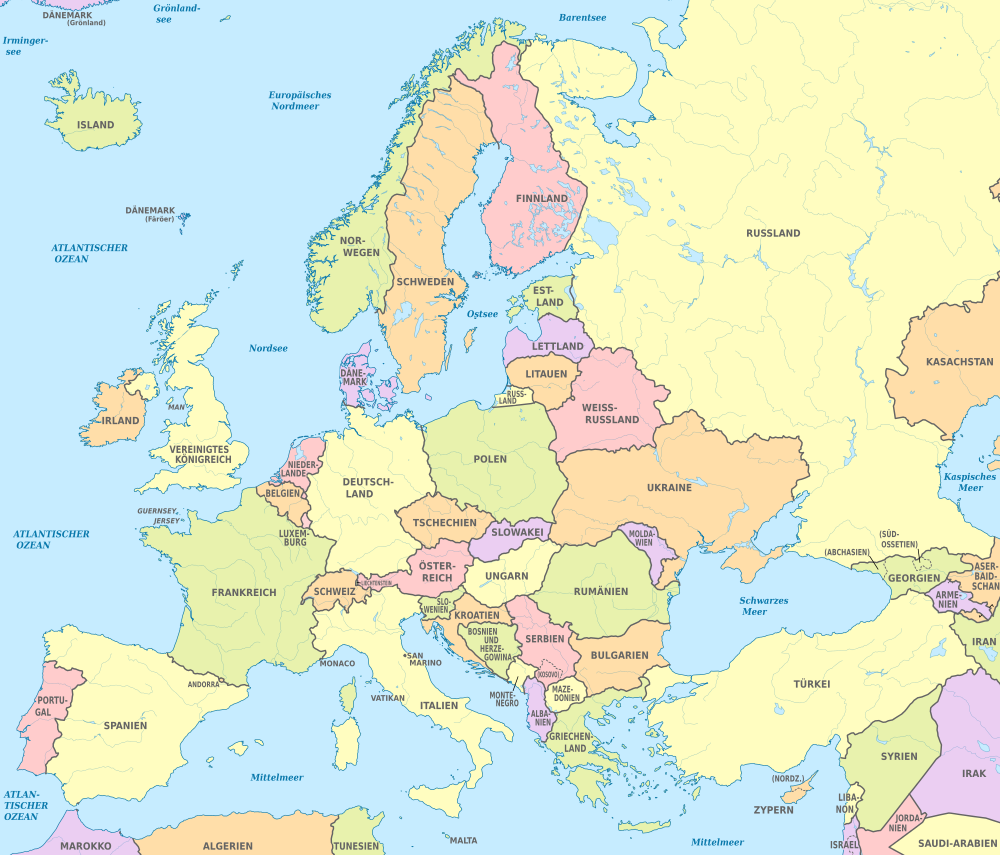
\includegraphics[width=.7\textwidth]{img/map_europe.png}
\end{center}
\end{frame}

\begin{frame}{Und noch eins}
\begin{center}
\chessboard[clearboard,setpieces={Qf8, Qc7, Qe6, Qh5, Qa4, Qd3, Qb2, Qg1}]
\end{center}
\end{frame}

\begin{frame}{Basics}
\begin{definition}[Constraint-Problem]
Ein \alert{Constraint-Problem} $(X, D, C)$ ist beschrieben durch
\begin{itemize}
  \item \emph{Variablen} $X$,
\emph{Domänen} $D = (D_x)_{x \in X}$ (endlich),
\emph{Constraints} $C$ 
\end{itemize} 

\end{definition}
\pause

Domänen typischerweise: \texttt{int}, \texttt{bool}, (\texttt{float})
\vspace*{2ex}

Was ist ein \textbf{Constraint}? Ein \emph{boolesches} Prädikat über einer Belegung von $X$:

$X = \{x, y, z \}$
\begin{itemize}
\item $x < y$
\item $x + 5 = z - y$
\item $\texttt{alldifferent}([x,y,z])$
\item $\forall$ und $\exists$ nur über endlichen Wertebereichen 
\end{itemize}
\end{frame} 
%
%\begin{frame}{Das eigentliche Erfüllbarkeitsproblem}
%Eine (partielle) Zuweisung ist eine (partielle) Abbildung $\theta : X \to D$ mit Scope $\mathrm{sc}$ als definierter Wertebereich.
%
%\begin{definition}[Lösung] 
%Eine Lösung für ein Constraint-Problem $(X, D, C)$
%ist eine Zuweisung $\theta$ mit $\mathrm{sc}(\theta) = X$, sodass $\theta$ alle Constraints $c \in C$ erfüllt, also
%$\forall c \in C : c(\theta) = \mathsf{tt}$.
%\end{definition}
%
%\vspace*{2ex}
%
%Ein Constraint-Satisfaction-Problem (CSP) besteht darin, eine Lösung $\theta$ aus dem Suchraum $[X \to D]$ zu finden~\cite{Rossi2006}.
%
%\end{frame}


\begin{frame}[fragile]{Beispiel}
\begin{columns}[onlytextwidth]
    \begin{column}{.48\textwidth}
     \hFirst{Problem}

CSP ($X$, $D$, $C$) mit 
\begin{itemize}
\item $X = \{x, y, z\}$
\item $D_x = D_y = \{0,1,2\}$, $D_z = \{0,1\}$
\item $C $
\begin{itemize}
\item $c_1 : x \neq y$, $y \neq z$, $x \neq z$
\item $c_2 : x + 1 = y$
\end{itemize}
\end{itemize}

    \pause 
    \end{column}
    \pause
    \begin{column}{.48\textwidth}
	\begin{lstlisting}
var 0..2: x;
var 0..2: y;
var 0..1: z;

% c1
constraint x != y /\ y != z /\ x != z;
% c2
constraint x + 1 = y;

solve satisfy;
\end{lstlisting}
    \end{column}
  \end{columns}
  
  \vspace*{3ex}
    \alert{Welche Zuweisung ist eine Lösung dieses Problems?}

\begin{itemize}
\item $\Theta = \{ (x \to 1, y \to 2, z \to ?), (x \to 0, y \to 1, z \to ?) \}$ erfüllen $c_2$; \pause
\item $(x \to 0, y \to 1, z \to ?)$ lässt sich aber zu keiner Lösung erweitern, da $z$ entweder 0 oder 1 sein muss und somit garantiert
$c_1$ verletzt \pause
\item Also ist die einzige Lösung $(x \to 1, y \to 2, z \to 0)$
\end{itemize}
\end{frame}
%\begin{frame}{Constraint-Algorithmen}
%Wesentliche Kernrichtungen für Algorithmen:
%
%\vspace*{2ex}
%
%\begin{itemize}
%\item \alert{Systematische} (vollständige) Suche (``\alert{Try}'')
%\begin{itemize}
%\item[-] Backtracking
%\item[-] Branch \& Bound
%\end{itemize} \pause
%
%\vspace*{1ex}
%
%\item Constraint-\alert{Propagation}, Inferenz
%\begin{itemize}
%\item[-] Einfache, lokale Konsistenzchecks (\emph{Logische Schlüsse})
%\item[-] \alert{Reduktion} der \emph{Domänen}
%\end{itemize} \pause
%
%\vspace*{1ex}
%
%\item \alert{Relaxierung}
%\begin{itemize}
%\item[-] Löse einfachere Teilprobleme
%\item[-] Nehme Ergebnis als \emph{Schranken}
%\end{itemize} \pause
%
%\vspace*{1ex}
%
%\item \alert{Lokale} (\emph{heuristische}) Suche
%\begin{itemize}
%\item[-] \emph{Min-Conflicts}-Heuristik
%\item[-] Large-neighborhood Search
%\item[-] Tabu-Suche / Simulated Annealing
%\end{itemize}
%\end{itemize}
%\end{frame}
%
%\begin{frame}{Systematische Suche}
%Partielle Zuweisungen schrittweise um ein Variablen-Wert-Paar erweitert.
%
%\vspace*{2ex}
%
%Ausnützen der Konjunktivität: Wenn eine partielle Zuweisung bereits \alert{einen} Constraint verletzt, wird die
%letzte Zuweisung \alert{rückgängig} gemacht (\emph{backtracking}) und neuer Wert versucht.
%
%\vspace*{2ex}
%
%Im schlimmsten Fall exponentielle Exploration aller vollständigen Zuweisungen $O(|D|^{|X|})$.
%
%\vspace*{1ex}
%
%$\rightarrow$ in der Praxis: 
%
%\begin{itemize}
%\item \textbf{Einschränkung der Lösungsraums durch \alert{Propagation}}
%\item Frühzeitiges Abschneiden von ``\alert{Sackgassen}''
%\item Frühzeitiges Probieren von \alert{vielversprechenden} Kandidaten
%\end{itemize}
%\end{frame}

\tikzstyle{sensor}=[draw, fill=blue!20, text width=5em, 
    text centered, minimum height=2.5em,drop shadow]    
    
\tikzstyle{alg} = [sensor, text width=5em, fill=isseorange!20, 
    minimum height=13em, rounded corners, drop shadow]
\tikzstyle{constraint}=[draw, circle, fill=issegrey!20, text width=1.2em, 
    text centered, minimum height=1.5em,drop shadow]
\tikzstyle{domainstore} = [alg, text width=5em, fill=isseorange!40, 
    minimum height=4em, rounded corners]
\tikzstyle{goodc} = [ForestGreen, font=\bfseries]
\tikzstyle{badc} = [Red, font=\bfseries]
\tikzstyle{okayc} = [LimeGreen, font=\bfseries]
        
\tikzset{
vecArrow/.style={
  thick
  }
}

\tikzset{
    mynode/.style={rectangle,rounded corners,draw=black, top color=isseorange!5, bottom color=isseorange!30,
                   very thick, inner sep=\myinnersep*1em, minimum size=3em, text centered, outer sep=0, align=center},
    innernode/.style={mynode, text width=3cm,  minimum height=1.5cm,
                      top color=issegrey!20, bottom color=issegrey!60},
    emphnode/.style={innernode, top color=isseorange!30, bottom color=isseorange!70}
}

% Define distances for bordering
\def\blockdist{2.3}
\def\edgedist{2.5}

  \tikzset{
    invisible/.style={opacity=0},
    visible on/.style={alt={#1{}{invisible}}},
    alt/.code args={<#1>#2#3}{%
      \alt<#1>{\pgfkeysalso{#2}}{\pgfkeysalso{#3}} % \pgfkeysalso doesn't change the path
    },
  }
  
\begin{frame}{Architektur von Constraint-Lösern}
\begin{center}
\begin{tikzpicture}
% First row:
 \node (search) [alg]  {Search \phantom{$x = 5$} };
 \path (search.east)+(4.6,0) node (propag) [alg,text width =12em]  {};
 \node[below right] at (propag.north west) {Constraint Store $C$};
 
 \path (propag.west)+(0.8,-1.2) node (c1) [constraint] {$c_1$}; 
 \path (propag.west)+(1.1,-0.2) node (c2) [constraint] {$c_2$}; 
 \path (propag.west)+(2.0,0.4) node (c3) [constraint] {$c_3$}; 
 \path (propag.west)+(3.2,0.7) node (c4) [constraint] {$c_4$};
  
 \path (propag.east)+(-1.2,-1.2) node (domainstore) [domainstore] {Domain Store $(D_x)_{x \in X}$}; 
 
 \path [draw,vecArrow, ->] ([yshift=-2em]search.north east) -- node [above,visible on=<2->] {$x\gets5$} ([yshift=-2em]propag.north west);
 \path [draw,vecArrow, <-] ([yshift=2em]search.south east) -- node [above,goodc,visible on=<4->] {$\top$} ([yshift=2em]propag.south west);
 
 \path [draw, vecArrow, <->] (c1.east) -- node [below,visible on=<3->,goodc] {$\top$} (domainstore.west) ;
 \path [draw,vecArrow, <->] (c2.330) -- node [above right,visible on=<3->,goodc] {$\top$} (domainstore.150) ;
 \path [draw,vecArrow, <->] (c3.290) -- node [right,visible on=<3->,goodc] {$\top$} (domainstore.120) ;
 \path [draw,vecArrow, <->] (c4.south) -- node [right,visible on=<3->,goodc] {$\top$} (domainstore.68) ;
\end{tikzpicture}
\end{center}

\end{frame}

\begin{frame}{Architektur von Constraint-Lösern}
\begin{center}
\begin{tikzpicture}
% First row:
 \node (search) [alg]  {Search $x = 5$};
 \path (search.east)+(4.6,0) node (propag) [alg,text width =12em]  {};
 \node[below right] at (propag.north west) {Constraint Store $C$};
 
 \path (propag.west)+(0.8,-1.2) node (c1) [constraint] {$c_1$}; 
 \path (propag.west)+(1.1,-0.2) node (c2) [constraint] {$c_2$}; 
 \path (propag.west)+(2.0,0.4) node (c3) [constraint] {$c_3$}; 
 \path (propag.west)+(3.2,0.7) node (c4) [constraint] {$c_4$};
  
 \path (propag.east)+(-1.2,-1.2) node (domainstore) [domainstore] {Domain Store $(D_x)_{x \in X}$}; 
 
 \path [draw,vecArrow, ->] ([yshift=-2em]search.north east) -- node [above,visible on=<2->] {$y \gets 4$} ([yshift=-2em]propag.north west);
 \path [draw,vecArrow, <-] ([yshift=2em]search.south east) -- node [below,badc,visible on=<4->] {$\bot$} ([yshift=2em]propag.south west);
 
 \path [draw, vecArrow, <->] (c1.east) -- node [below,visible on=<3->,badc] {$\bot$} (domainstore.west) ;
 \path [draw,vecArrow, <->] (c2.330) -- node [above right,visible on=<3->,goodc] {$\top$} (domainstore.150) ;
 \path [draw,vecArrow, <->] (c3.290) -- node [right,visible on=<3->,goodc] {$\top$} (domainstore.120) ;
 \path [draw,vecArrow, <->] (c4.south) -- node [right,visible on=<3->,goodc] {$\top$} (domainstore.68) ;
\end{tikzpicture}
\end{center}
\end{frame}
%
%\begin{frame}{Constraint-Propagation}
%\begin{itemize}
%\item Nutze Constraints, um Suchraum einzugrenzen
%\item Idee: Entferne alle Werte aus Domänen, die in keiner
%Lösung vorkommen können (\emph{Domain Store}) \pause
%\item $|x_1 - x_2| > 5$ für $x_1, x_2 \in X$ und $D_{x_i} = \{1,\ldots, 10\}$
%\item \alert{Welche Werte sind nicht möglich?} \alert
%\item jeweils 5 und 6 \pause
%\item Propagierungsschritte beeinflussen einander
%\begin{itemize}
%\item ``Kettenreaktion''
%\item Fixpunktalgorithmus $\rightarrow$ Keine Propagierung möglich
%\item Wenn Domäne nur mehr einen Wert enthält, \emph{muss} dieser
%zugewiesen werden.
%\end{itemize}
%\end{itemize}
%\end{frame}

\begin{frame}{Constraint-Propagation: Beispiel}
\begin{center}
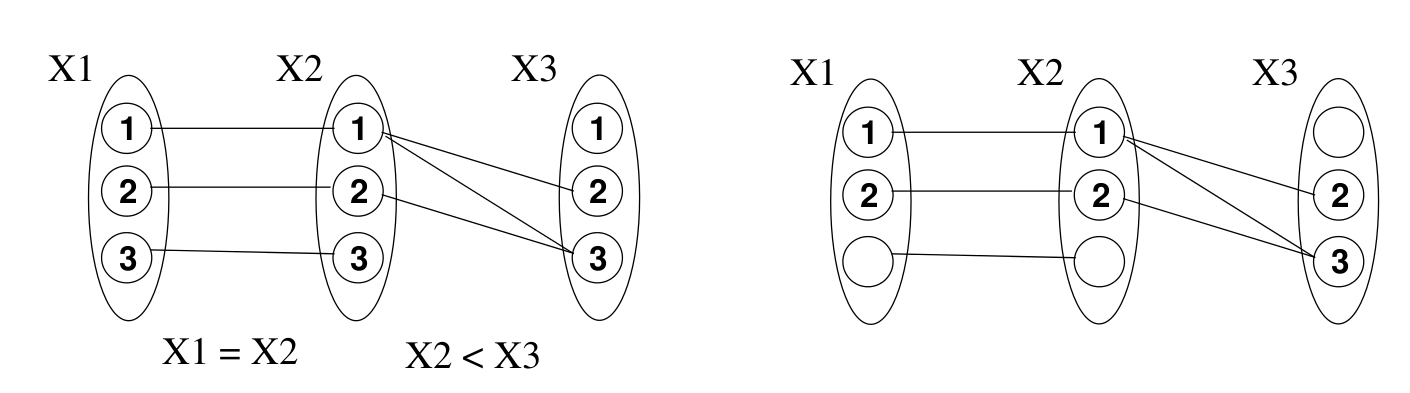
\includegraphics[width=\textwidth]{img/constprop.png}
\end{center}
Entfernen von Werten, die zu keiner Lösung führen können. 
\end{frame}


\begin{frame}{Globale Constraints}
\begin{itemize}
\item Betrachten wir folgendes einfaches Problem
\begin{itemize}
\item $X = \{x_1, x_2, x_3 \}$
\item $(D_x)_{x \in X} = \{1,2\}$
\item $C$ : $x_1 \neq x_2$, $x_2 \neq x_3$, $x_1 \neq x_3$
\end{itemize}
\item Ist dieses Problem nach Constraint-Propagation mit binären Constraints \alert{lösbar}? \pause
\item Ja, für jedes $d \in D_x$ gibt es einen Partner \pause 
\item Insgesamt allerdings nicht, da mindestens 3 unterschiedliche Werte nötig
\item $\rightarrow$ daher globale Constraints, die eine größere Menge von Variablen im Auge betrachten können
\item Und \emph{spezialisierte} Propagationsalgorithmen haben!
\item $\mathtt{alldifferent(x_1, x_2, x_3)}$
\end{itemize}
\end{frame}

\begin{frame}{Task-Zuweisung in Practice}
\begin{itemize}
\item Taskzuweisungsproblem (\emph{task allocation problem})

\begin{itemize}
\item [-] $n$ Roboter
\item [-] $m$ Tasks
\item [-] Gebe jedem Roboter einen \emph{unterschiedlichen} Task, um den Gewinn zu maximieren (Unterschied zu Kompensation und Strafe)
\end{itemize}
\item Beispielproblem:
\begin{itemize}
\item[-] $n = 4$, $m = 5$
\end{itemize}
\end{itemize}
\centering
\begin{tabular}{|c|c|c|c|c|c|}
\hline 
 & t1 & t2 & t3 & t4 & t5 \\ 
\hline 
r1 & 7 & 1 & 3 & 4 & 6 \\ 
\hline 
r2 & 8 & 2 & 5 & 1 & 4 \\ 
\hline 
r3 & 4 & 3 & 7 & 2 & 5 \\ 
\hline 
r4 & 3 & 1 & 6 & 3 & 6 \\ 
\hline 
\end{tabular} 
\end{frame}


\begin{frame}[fragile]{Task-Zuweisung: Modell}
\begin{lstlisting}
% problem data 
int: n; set of int: ROBOTS = 1..n;
int: m; set of int: TASKS = 1..m;
array[ROBOTS,TASKS] of int: profit;

% decisions
array[ROBOTS] of var TASKS: allocation;

% goal
solve maximize sum(r in ROBOTS) (profit[r, allocation[r]] );

% have robots work on different tasks
constraint alldifferent(allocation);
\end{lstlisting}
\end{frame}

\begin{frame}[fragile]{AllDifferent -- Machbarkeit}
\begin{itemize}
\item Erster bekannter Propagator
\item Basiert auf Matching in bipartiten Graphen
\item Laufzeit ist polynomiell!
\end{itemize}

\begin{lstlisting}
var {1,2,3}: x;       var {2,3}: y;      var {2,3}: z;
var {1,2,3,4,5}: t; var {3,4,5,6}: u;
constraint alldifferent([x,y,z,t,u]);
\end{lstlisting}
\vspace*{-15ex}
\begin{center}
\tikzset{onslide/.code args={<#1>#2}{%
  \only<#1>{\pgfkeysalso{#2}}
}}
\tikzstyle{highlight}=[isseorange,ultra thick]
\begin{tikzpicture}[every node/.style={
anchor=base,
text depth=.5ex,
text height=2ex,
minimum height=2ex,
align=center,
circle,
text width=1em}]
\matrix (magic) [nodes in empty cells, ampersand replacement=\&,row sep=0.3cm,column sep=0.5cm]
{
\node[draw, circle](x){$x$}; \& \node[draw, circle](y){$y$};  \& \node[draw, circle](z){$z$};  \& \node[draw, circle](t){$t$};  \& \node[draw, circle](u){$u$};  \\
 \& \\
\& \\
\& \\
\node[draw, circle](1){$1$};  \& \node[draw, circle](2){$2$};  \& \node[draw, circle](3){$3$};  \& \node[draw, circle](4){$4$};  \& \node[draw, circle](5){$5$};  \& \node[draw, circle](6){$6$};  \\
};

\draw[onslide={<2>{highlight}}] (x) -- (1);
\draw[] (x) -- (2);
\draw[] (x) -- (3);

\draw[onslide={<2>{highlight}}] (y) -- (3);
\draw[] (y) -- (2);

\draw[onslide={<2>{highlight}}] (z) -- (2);
\draw[] (z) -- (3);

\draw[onslide={<2>{highlight}}] (t) -- (5);
\draw[] (t) -- (1);
\draw[] (t) -- (2);
\draw[] (t) -- (3);
\draw[] (t) -- (4);
\draw[onslide={<2>{highlight}}] (u) -- (4);
\draw[] (u) -- (3);
\draw[] (u) -- (5);
\draw[] (u) -- (6);
\end{tikzpicture}
\end{center}

\end{frame}

\begin{frame}[fragile]{AllDifferent -- Propagierung}

\begin{lstlisting}
var {1,2,3}: x;       var {2,3}: y;      var {2,3}: z;
var {1,2,3,4,5}: t; var {3,4,5,6}: u;
constraint alldifferent([x,y,z,t,u]);
\end{lstlisting}
\vspace*{-15ex}
\begin{center}
\tikzset{onslide/.code args={<#1>#2}{%
  \only<#1>{\pgfkeysalso{#2}}
}}
\tikzstyle{highlight}=[isseorange,ultra thick]
\tikzstyle{impo}=[dashed]
\begin{tikzpicture}[every node/.style={
anchor=base,
text depth=.5ex,
text height=2ex,
minimum height=2ex,
align=center,
circle,
text width=1em}]
\matrix (magic) [nodes in empty cells, ampersand replacement=\&,row sep=0.3cm,column sep=0.5cm]
{
\node[draw, circle](x){$x$}; \& \node[draw, circle](y){$y$};  \& \node[draw, circle](z){$z$};  \& \node[draw, circle](t){$t$};  \& \node[draw, circle](u){$u$};  \\
 \& \\
\& \\
\& \\
\node[draw, circle](1){$1$};  \& \node[draw, circle](2){$2$};  \& \node[draw, circle](3){$3$};  \& \node[draw, circle](4){$4$};  \& \node[draw, circle](5){$5$};  \& \node[draw, circle](6){$6$};  \\
};

\draw[onslide={<2>{highlight}}] (x) -- (1);
\draw[onslide={<2>{impo}}] (x) -- (2);
\draw[onslide={<2>{impo}}] (x) -- (3);

\draw[onslide={<2>{highlight}}] (y) -- (3);
\draw[] (y) -- (2);

\draw[onslide={<2>{highlight}}] (z) -- (2);
\draw[] (z) -- (3);

\draw[onslide={<2>{highlight}}] (t) -- (5);
\draw[onslide={<2>{impo}}] (t) -- (1);
\draw[onslide={<2>{impo}}] (t) -- (2);
\draw[onslide={<2>{impo}}] (t) -- (3);
\draw[] (t) -- (4);
\draw[onslide={<2>{highlight}}] (u) -- (4);
\draw[onslide={<2>{impo}}] (u) -- (3);
\draw[] (u) -- (5);
\draw[] (u) -- (6);
\end{tikzpicture}
\end{center}
\vspace*{-15ex}
\begin{lstlisting}
var {1}: x;       var {2,3}: y;      var {2,3}: z;
var {4,5}: t;      var {4,5,6}: u;
constraint alldifferent([x,y,z,t,u]);
\end{lstlisting}
\end{frame}

\begin{frame}[fragile]{AllDifferent -- Algorithmus}

\begin{lstlisting}
var {1,2,3}: x;       var {2,3}: y;      var {2,3}: z;
var {1,2,3,4,5}: t; var {3,4,5,6}: u;
constraint alldifferent([x,y,z,t,u]);
\end{lstlisting}
\vspace*{-15ex}
\begin{center}
\tikzset{onslide/.code args={<#1>#2}{%
  \only<#1>{\pgfkeysalso{#2}}
}}
\tikzstyle{highlight}=[isseorange,ultra thick]
\tikzstyle{impo}=[dashed]
\begin{tikzpicture}[every node/.style={
anchor=base,
text depth=.5ex,
text height=2ex,
minimum height=2ex,
align=center,
circle,
text width=1em}]
\matrix (magic) [nodes in empty cells, ampersand replacement=\&,row sep=0.3cm,column sep=0.5cm]
{
\node[draw, circle](x){$x$}; \& \node[draw,onslide={<2->{highlight}}, circle](y){$y$};  \& \node[draw, onslide={<2->{highlight}}, circle](z){$z$};  \& \node[draw, onslide={<2->{highlight}}, circle](t){$t$};  \& \node[draw, circle](u){$u$};  \\
 \& \\
\& \\
\& \\
\node[draw, circle](1){$1$};  \& \node[draw, onslide={<2->{highlight}}, circle](2){$2$};  \& \node[draw, onslide={<2->{highlight}}, circle](3){$3$};  \& \node[draw, circle](4){$4$};  \& \node[draw, onslide={<2->{highlight}},circle](5){$5$};  \& \node[draw, circle](6){$6$};  \\
};

\draw[onslide={<1->{highlight}}] (x) -- (1);
\draw[] (x) -- (2);
\draw[] (x) -- (3);

\draw[onslide={<3>{highlight}}] (y) -- (3);
\draw[] (y) -- (2);

\draw[onslide={<1-2>{highlight}}] (z) -- (3);
\draw[onslide={<3>{highlight}}] (z) -- (2);

\draw[onslide={<1-2>{highlight}}] (t) -- (2);
\draw[] (t) -- (1);
\draw[onslide={<3>{highlight}}] (t) -- (5);
\draw[] (t) -- (3);
\draw[] (t) -- (4);
\draw[onslide={<1>{highlight}}] (u) -- (4);
\draw[] (u) -- (3);
\draw[] (u) -- (5);
\draw[] (u) -- (6);
\end{tikzpicture}
\end{center}
\vspace*{-15ex}
Augmentierender Pfad:

$y \to 3 \to z \to 2 \to t \to 5$
\end{frame}

\begin{frame}{Let that sink in}

\begin{parchment}[Take away message]
\large
\alert{Global constraints} are the \alert{essence} of constraint programming!
\end{parchment}
\end{frame}

\tikzset{
    process/.style={rectangle,rounded corners,draw=black, top color=isseorange!5, bottom color=isseorange!30},
    file/.style={rectangle,draw=black}
}

\begin{frame}{How can we actually use all that?}
\alert{Architecture}

\begin{center}
\vspace*{-25ex}
\begin{tikzpicture}[every node/.style={
anchor=base,
text depth=.5ex,
text height=2ex,
minimum height=2ex,
align=center,
circle,
minimum width=1em}]
\matrix (magic) [nodes in empty cells, ampersand replacement=\&,row sep=0.3cm,column sep=0.5cm]
{
\node[draw, file,isseorange,thick](cr){\texttt{cr.dzn}};  \\
\node[draw, file](f1){\texttt{f1.dzn}}; \& \& \node[draw, process](mzn2fzn){\texttt{mzn2fzn}}; \& \& \node[draw, file](output){\emph{output}};  \\
\node[draw, file](f2){\texttt{f2.dzn}};   \&  \&  \node(inv){}; \& \node[draw, rectangle, rounded corners](globals){solver-specific globals};  \\
\node[draw, file](mod){\texttt{model.mzn}}; \& \&  \\
\& \& \node[draw, file](fzn){\texttt{compiled.fzn}}; \& \& \node[draw, process](solve){\texttt{solve}};  \\
\& \\
};

\draw[dashed,->] (f1) -- (mzn2fzn);
\draw[dashed,->] (f2) -- (mzn2fzn);
\draw[dashed,->] (cr) -- (mzn2fzn);
\draw[dashed,->] (mod) -- (mzn2fzn);
\draw[dashed,->] (fzn) -- (solve);
\draw[->] (mzn2fzn) -- (fzn);
\draw[->] (solve) -- (output);
\draw[dashed] (globals) -- (inv);
\end{tikzpicture}
\end{center}
\vspace*{-25ex}

\end{frame}

\begin{frame}{Why MiniZinc?}
\begin{parchment}[Rationale]
\centering 
\alert{One modeling language -- many solvers} 
\end{parchment}
\begin{textblock*}{2.cm}[1,1](\textwidth-.5cm,\textheight-1.03cm)


\includegraphics[width=\textwidth]{img/MiniZn_logo.jpg} 

\end{textblock*}
Supported Solvers
\begin{itemize}
\item Gecode (CP)
\item JaCoP (CP)
\item Google Optimization Tools (CP)
\item Choco (CP)
\item G12 (CP/LP/MIP)
\end{itemize}

\end{frame}

%\begin{frame}[fragile]{Globale Constraints: Beispiele}
%Häufig auftretende Constraints samt Propagierungsalgorithmen. Gesammelt im \emph{Global Constraints Catalogue}\footnote{\url{http://www.emn.fr/z-info/sdemasse/gccat/sec5.html}}
%
%\vspace*{2ex}
%
%\begin{description}
%\item[{\tt \textbf{alldifferent(VARIABLES)}}] Erfordert, dass alle Variablen \alert{unterschiedliche} Werte haben, z.B: $[1,2,3]$ \pause
%
%\item[{\tt \textbf{allequal(VARIABLES)}}] Erfordert, dass alle Variablen den \alert{gleichen} Wert haben, z.B: $[5,5,5]$ \pause
%
%\item[{\tt \textbf{nvalue(VARIABLES, N)}}] Erfordert, dass genau $N$ verschiedene Werte vorkommen, z.B: $([1,2,1],2)$ \pause
%
%\item[{\tt \textbf{at\_most(N, VARIABLES, V)}}] Erfordert, dass höchstens $N$ Variablen den Wert $V$ annehmen z.B: $(2,[2,2,4],2)$
%
%
%\end{description}
%\end{frame}

\begin{frame}{Scheduling \& Packing}
\begin{itemize}
\item A very important application for CP
\item Strong support (global constraints) in MiniZinc
\begin{itemize}
\item[-] Involved propagators -- fortunately encapsulated by solvers!
\end{itemize}
\vspace*{1ex}

\item Planning and scheduling are coming together and constraint
satisfaction may serve as a bridge between them
\item Many applications in practice (production style problems)

\vspace*{1ex}
\item Overview papers:
\begin{itemize}
\item Bartak'03~\cite{Bartak03constraintbasedscheduling}
\item Bartak'10~\cite{bartak2010constraint}
\item Baptiste'06~\cite{baptiste2006constraint}
\end{itemize}
\end{itemize}
\end{frame}

\begin{frame}[fragile]{Intro to Scheduling}
\tikzset{
    task/.style={rounded corners, minimum height=3.8ex,rectangle,anchor=south west},
    task1/.style={task,draw=black, top color=isseorange!5, bottom color=isseorange!30},    
    task2/.style={task,draw=black, top color=ForestGreen!5, bottom color=ForestGreen!30},
    task3/.style={task,draw=black, top color=BrickRed!5, bottom color=BrickRed!30},
} 
\vspace*{-6ex}
\begin{figure}
\begin{tikzpicture}[scale=1.0]
    % Draw axes
    \draw [<->,thick] (0,3) node (yaxis) [above] {Workers}
        |- (8.5,0) node (xaxis) [right] {$t$};    
    
% first slide

\onslide<1>{
    \node[task1] at (-3,2.1) { cut onions };        
    \node[task2] at (-3,1.4) { cook onions };          
    \node[task3] at (-3,0.7) { cook spaghetti };  
}
    
\onslide<2->{    
    \node[task1] at (2,0.5) { cut onions };        
    \node[task2] at (4,0.5) { cook onions };          
    \node[task3] at (2,1.5) { cook spaghetti };  
}

\onslide<3->{
	\node at (1.5,1.75) {\footnotesize \texttt{s[t]}};  
	}

\onslide<5->{
	\node at (4.85,1.75) {\footnotesize \texttt{e[t]}};  
}

\onslide<4->{	
\draw [decorate,decoration={brace,amplitude=10pt,raise=4pt},yshift=0pt]
(2,2.0) -- (4.3,2.0) node [black,midway,yshift=20pt] {\footnotesize \texttt{dur[t]}};
    }
    
    \node[text centered, anchor=center] at (-0.3,0.8) { $P_1$ }; \draw[thick] (-0.1,0.8) -- (0.1,0.8);
	\node[text centered, anchor=center] at (-0.3,1.8) { $P_2$ }; \draw[thick] (-0.1,1.8) -- (0.1,1.8);
	
	\node[text centered, anchor=north] at (1,0) { 1 }; \draw[thick] (1,0.05) -- (1,-.05);
	\node[text centered, anchor=north] at (2,0) { 2 }; \draw[thick] (2,0.05) -- (2,-.05);
	\node[text centered, anchor=north] at (3,0) { 3 }; \draw[thick] (3,0.05) -- (3,-.05);	
	\node[text centered, anchor=north] at (4,0) { 4 }; \draw[thick] (4,0.05) -- (4,-.05);
	\node[text centered, anchor=north] at (5,0) { 5 }; \draw[thick] (5,0.05) -- (5,-.05);
	\node[text centered, anchor=north] at (6,0) { 6 }; \draw[thick] (6,0.05) -- (6,-.05);
	\node[text centered, anchor=north] at (7,0) { 7 }; \draw[thick] (7,0.05) -- (7,-.05);	
	\node[text centered, anchor=north] at (8,0) { 8 }; \draw[thick] (8,0.05) -- (8,-.05);
	   
\end{tikzpicture}
\end{figure}

\pause \pause \pause \pause \pause

\begin{lstlisting}
int: T; set of int: TASK = 1..T; set of int: HORIZON = 0..10;

array[TASK] of var HORIZON: s; % start times
array[TASK] of var HORIZON: e; % end times 
array[TASK] of HORIZON: du;    % durations (fixed as constants!)

constraint forall(t in TASK) (s[t] + du[t] = e[t]); % consistency
constraint e[cut_on] <= s[cook_on]; % precedence
\end{lstlisting}

\end{frame}
\begin{frame}[fragile]{Non-overlaps (Manually)}

\tikzset{
    task/.style={rounded corners, minimum height=3.8ex,rectangle,anchor=south west},
    task1/.style={task,draw=black, top color=isseorange!5, bottom color=isseorange!30},    
    task2/.style={task,draw=black, top color=issegrey!5, bottom color=issegrey!30},
    task3/.style={task,draw=black, top color=BrickRed!5, bottom color=BrickRed!30},
}
 
%\vspace*{-6ex}
\begin{figure}
\begin{tikzpicture}[scale=1.0]
    % Draw axes
    \draw [<->,thick] (0,2) node (yaxis) [above] {}
        |- (4.0,0) node (xaxis) [right] {$t$};    

    \draw [<->,thick] (6,2) node (yaxis) [above] {}
        |- (10.0,0) node (xaxis) [right] {$t$};      
% first slide

    \node[task1] at (1,0.5) { cut onions };        
    \node[task2] at (1.5,1.1) { cook onions };         

    \node[task1] at (6,0.5) { cut onions };        
    \node[task2] at (8,1.1) { cook onions };          
 
  %  \node[task3] at (2,1.5) { cook spaghetti };  

	\node at (1.9, 2.6) {\color{BrickRed} \Huge \Lightning };
	\node at (7.9, 2.6) {\color{ForestGreen} \Huge \checkmark };
	
	\node[text centered, anchor=north] at (1,0) { 1 }; \draw[thick] (1,0.05) -- (1,-.05);
	\node[text centered, anchor=north] at (2,0) { 2 }; \draw[thick] (2,0.05) -- (2,-.05);
	\node[text centered, anchor=north] at (3,0) { 3 }; \draw[thick] (3,0.05) -- (3,-.05);	
%	\node[text centered, anchor=north] at (4,0) { 4 }; \draw[thick] (4,0.05) -- (4,-.05);
	\node[text centered, anchor=north] at (7,0) { 1 }; \draw[thick] (7,0.05) -- (7,-.05);	
	\node[text centered, anchor=north] at (8,0) { 2 }; \draw[thick] (8,0.05) -- (8,-.05);
	\node[text centered, anchor=north] at (9,0) { 3 }; \draw[thick] (9,0.05) -- (9,-.05);
	   
\end{tikzpicture}
\end{figure}

\begin{lstlisting}
predicate nonoverlap(var TASK: task1, var TASK: task2) = 
             s[task1] + d[task1] <= s[task2] \/ 
             s[task2] + d[task2] <= s[task1];
             
             
constraint nonoverlap(cut_on, cook_on);
\end{lstlisting}
\end{frame}

\begin{frame}[fragile]{Non-overlaps (Global Constraint)}

\tikzset{
    task/.style={rounded corners, minimum height=3.8ex,rectangle,anchor=south west},
    task1/.style={task,draw=black, top color=isseorange!5, bottom color=isseorange!30},    
    task2/.style={task,draw=black, top color=issegrey!5, bottom color=issegrey!30},
    task3/.style={task,draw=black, top color=BrickRed!5, bottom color=BrickRed!30},
}
 
%\vspace*{-6ex}
\begin{figure}
\begin{tikzpicture}[scale=1.0]
    % Draw axes
    \draw [<->,thick] (0,2) node (yaxis) [above] {}
        |- (4.0,0) node (xaxis) [right] {$t$};    

    \draw [<->,thick] (6,2) node (yaxis) [above] {}
        |- (10.0,0) node (xaxis) [right] {$t$};      
% first slide

    \node[task1] at (1,0.5) { cut onions };        
    \node[task2] at (1.5,1.1) { cook onions };         

    \node[task1] at (6,0.5) { cut onions };        
    \node[task2] at (8,1.1) { cook onions };          
 
  %  \node[task3] at (2,1.5) { cook spaghetti };  

	\node at (1.9, 2.6) {\color{BrickRed} \Huge \Lightning };
	\node at (7.9, 2.6) {\color{ForestGreen} \Huge \checkmark };
	
	\node[text centered, anchor=north] at (1,0) { 1 }; \draw[thick] (1,0.05) -- (1,-.05);
	\node[text centered, anchor=north] at (2,0) { 2 }; \draw[thick] (2,0.05) -- (2,-.05);
	\node[text centered, anchor=north] at (3,0) { 3 }; \draw[thick] (3,0.05) -- (3,-.05);	
%	\node[text centered, anchor=north] at (4,0) { 4 }; \draw[thick] (4,0.05) -- (4,-.05);
	\node[text centered, anchor=north] at (7,0) { 1 }; \draw[thick] (7,0.05) -- (7,-.05);	
	\node[text centered, anchor=north] at (8,0) { 2 }; \draw[thick] (8,0.05) -- (8,-.05);
	\node[text centered, anchor=north] at (9,0) { 3 }; \draw[thick] (9,0.05) -- (9,-.05);
	   
\end{tikzpicture}
\end{figure}

\begin{lstlisting}
include "disjunctive.mzn"; % global definition from standard library
predicate disjunctive(array [int] of var int: s,
                      array [int] of var int: d)
             
constraint nonoverlap( [ s[cut_on], s[cook_on] ], 
                          [ du[cut_on], du[cook_on] ]);
\end{lstlisting}
\end{frame}


\begin{frame}{A small example}
\begin{center}

\includegraphics[width=.15\textwidth]{img/boy1.png} \qquad \qquad

\includegraphics[width=.15\textwidth]{img/boy2.png}

\vspace*{3ex}


\includegraphics[width=.15\textwidth]{img/computer.png} \qquad \qquad

\includegraphics[width=.15\textwidth]{img/mother.png}
\end{center}

\begin{itemize}
\item Two brothers, Alfred and Ben; both need to 
\begin{itemize}
\item[-] Read about an algorithm before
\item[-] programming it on a computer
\end{itemize}
\item Their mother needs to do work on a computer as well
\item Only one computer is available
\end{itemize}
\end{frame}

\begin{frame}[fragile]{Model}

\begin{lstlisting}
int: T = 5; set of int: TASK = 1..T;
set of int: HORIZON = 0..50;
array[TASK] of var HORIZON: s; % start times
array[TASK] of var HORIZON: e; % end times 
var HORIZON: makeSpan; 
int: readAlfred = 1; int: codeAlfred = 2;
int: readBen = 3; int: codeBen = 4; int: workMother = 5;

% durations
array[TASK] of int: d = [5, 2, 3, 8, 12];

constraint forall(t in TASK) (s[t] + d[t] = e[t]);
constraint forall(t in TASK) (e[t] <= makeSpan);
constraint e[readAlfred] <= s[codeAlfred] /\ e[readBen] <= s[codeBen];

set of TASK: conflicting = {codeAlfred, codeBen, workMother};
constraint disjunctive( [s[t] | t in conflicting], 
                         [d[t] | t in conflicting] ); 
solve minimize makeSpan;
\end{lstlisting}
\end{frame}

\begin{frame}[fragile]{Solution}

\begin{lstlisting}
int: readAlfred = 1; int: codeAlfred = 2;
int: readBen = 3; int: codeBen = 4; int: workMother = 5;
set of TASK: conflicting = {codeAlfred, codeBen, workMother};
array[TASK] of int: d = [5, 2, 3, 8, 12];
\end{lstlisting}
\small 
\begin{verbatim}
s = array1d(1..5 ,[0, 20, 0, 12, 0]);
e = array1d(1..5 ,[5, 22, 3, 20, 12]);
makeSpan = 22;
\end{verbatim}

\tikzset{
    task/.style={rounded corners, text centered, minimum height=3.8ex,rectangle,anchor=south west},
    task1/.style={task,draw=black, top color=isseorange!5, bottom color=isseorange!30},    
    task2/.style={task,draw=black, top color=ForestGreen!5, bottom color=ForestGreen!30},
    task3/.style={task,draw=black, top color=BrickRed!5, bottom color=BrickRed!30},
}
 \hspace*{-2ex}
 \begin{tikzpicture}[x=1cm,y=1cm]
    % Draw axes
    \draw [<->,thick] (0,2.7) node (yaxis) [above] {}
        |- (11.65,0) node (xaxis) [right] {$t$};    

  %  \node[task1] at (1,0.5) { cut onions };        
    \node[task2,text width=2.8cm] at (0,0.3) {read (A)};         
    \node[task2,text width=1.8cm] at (0,0.9) {read (B)};         

    \node[task3,text width=4.8cm] at (0,1.5) {work (mother)};         
	\node[task3,text width=2.4cm] at (9,0.3) {code (A)};         
    \node[task3,text width=3.8cm] at (5,0.9) {code (B)};        
   
  %  \node[task3] at (2,1.5) { cook spaghetti };  

\end{tikzpicture}
 
\end{frame}


 
 \begin{frame}{Cumulative Scheduling}
\begin{itemize}
\item \texttt{disjunctive} is useful for \alert{unary} resources
\item It is actually a special case of \texttt{cumulative}
\begin{itemize}
\item I have $m$ copies of the same resource
\item No more than $m$ can be used at once!
\item Example: $m$ workers, $m$ bulldozers, $m$ tools, \ldots
\end{itemize}
\vspace*{2ex}

\item Assume task \texttt{t} takes \texttt{res[t]} resources
\end{itemize}

\tikzset{
    task/.style={rounded corners, minimum height=3.8ex,rectangle,anchor=south west},
    task1/.style={task,draw=black, top color=isseorange!5, bottom color=isseorange!30},    
    task2/.style={task,draw=black, top color=issegrey!5, bottom color=issegrey!30},
    task3/.style={task,draw=black, top color=BrickRed!5, bottom color=BrickRed!30},
}
 
%\vspace*{-6ex}
\begin{figure}
\begin{tikzpicture}[scale=1.0,x=1cm,y=1cm]
    % Draw axes
    \draw [<->,thick] (0,3.2) node (yaxis) [above] {\texttt{res[t]}}
        |- (5.5,0) node (xaxis) [right] {$t$};    

    \draw [<->,thick] (6,3.2) node (yaxis) [above] {\texttt{res[t]}}
        |- (11.5,0) node (xaxis) [right] {$t$};      
% first slide
 
    \node[task1,text width=1.8cm,text height=2cm] at (0,0) {  };        
    \node[task1,text width=2.3cm,text height=.5cm] at (0,2.25) { };         
    \node[task1,text width=2.5cm,text height=.2cm] at (2.05,0) {  }; 
    \node[task1,text width=1.cm,text height=.2cm] at (2.05,0.6) {  };         
   
    \node[task1,text width=1.8cm,text height=2cm] at (6,0) {  };        
    \node[task1,text width=2.3cm,text height=.5cm] at (8.05,1.2) { };         
    \node[task1,text width=2.5cm,text height=.2cm] at (8.05,0) {  }; 
    \node[task1,text width=1.cm,text height=.2cm] at (8.05,0.6) {  };    
  %  \node[task3] at (2,1.5) { cook spaghetti };  

\node at (1.9, 3.4) {\color{BrickRed} \Huge \Lightning };
	\node at (7.9, 3.4) {\color{ForestGreen} \Huge \checkmark };
	
	
 \draw [dashed,BrickRed,very thick] (-0.3,2.25) -- (11,2.25) ;
	   
\end{tikzpicture}
\end{figure}
\end{frame}

\begin{frame}[fragile]{Cumulative Global Constraint}



\begin{lstlisting}
predicate cumulative(array [int] of var int: s,
                       array [int] of var int: d,
                       array [int] of var int: r,
                       var int: b)
\end{lstlisting}

\begin{parchment}[MiniZinc Docs]
Requires that a set of tasks given by start times \texttt{s}, durations \texttt{d}, and resource requirements \texttt{r}, never require more than a global resource bound \texttt{b} at any one time.
\end{parchment}
\end{frame}


\begin{frame}[fragile]{Household Revisited}
How about buying a new computer? 
\begin{lstlisting}
predicate cumulative(array [int] of var int: s,
                       array [int] of var int: d,
                       array [int] of var int: r,
                       var int: b)
\end{lstlisting}

\begin{lstlisting}
set of TASK: conflicting = {codeAlfred, codeBen, workMother};
int: nComputers = 2;

constraint cumulative( [ s[t] | t in conflicting], 
                          [ d[t] | t in conflicting], 
                          [ 1   | t in conflicting], 
                          nComputers ); 
\end{lstlisting}

\end{frame}

\begin{frame}[fragile]{Solution (1 Computer)}

\begin{lstlisting}
int: readAlfred = 1; int: codeAlfred = 2;
int: readBen = 3; int: codeBen = 4; int: workMother = 5;
set of TASK: conflicting = {codeAlfred, codeBen, workMother};
array[TASK] of int: d = [5, 2, 3, 8, 12];
\end{lstlisting}
\small 
\begin{verbatim}
s = array1d(1..5 ,[0, 20, 0, 12, 0]);
e = array1d(1..5 ,[5, 22, 3, 20, 12]);
makeSpan = 22;
\end{verbatim}

\tikzset{
    task/.style={rounded corners, text centered, minimum height=3.8ex,rectangle,anchor=south west},
    task1/.style={task,draw=black, top color=isseorange!5, bottom color=isseorange!30},    
    task2/.style={task,draw=black, top color=ForestGreen!5, bottom color=ForestGreen!30},
    task3/.style={task,draw=black, top color=BrickRed!5, bottom color=BrickRed!30},
}
 \hspace*{-2ex}
 \begin{tikzpicture}[x=1cm,y=1cm]
    % Draw axes
    \draw [<->,thick] (0,2.7) node (yaxis) [above] {}
        |- (11.65,0) node (xaxis) [right] {$t$};    

  %  \node[task1] at (1,0.5) { cut onions };        
    \node[task2,text width=2.8cm] at (0,0.3) {read (A)};         
    \node[task2,text width=1.8cm] at (0,0.9) {read (B)};         

    \node[task3,text width=4.8cm] at (0,1.5) {work (mother)};         
	\node[task3,text width=2.4cm] at (9,0.3) {code (A)};         
    \node[task3,text width=3.8cm] at (5,0.9) {code (B)};        
   
  %  \node[task3] at (2,1.5) { cook spaghetti };  

\end{tikzpicture}
 
\end{frame}


\begin{frame}[fragile]{Solution (2 Computers)}

\begin{lstlisting}
int: readAlfred = 1; int: codeAlfred = 2;
int: readBen = 3; int: codeBen = 4; int: workMother = 5;
set of TASK: conflicting = {codeAlfred, codeBen, workMother};
array[TASK] of int: d = [5, 2, 3, 8, 12];
\end{lstlisting}
\small 
\begin{verbatim}
s = array1d(1..5 ,[0, 11, 0, 3, 0]);
e = array1d(1..5 ,[5, 13, 3, 11, 12]);
makeSpan = 13;
\end{verbatim}

\tikzset{
    task/.style={rounded corners, text centered, minimum height=3.8ex,rectangle,anchor=south west},
    task1/.style={task,draw=black, top color=isseorange!5, bottom color=isseorange!30},    
    task2/.style={task,draw=black, top color=ForestGreen!5, bottom color=ForestGreen!30},
    task3/.style={task,draw=black, top color=BrickRed!5, bottom color=BrickRed!30},
}
 \hspace*{-2ex}
 \begin{tikzpicture}[x=1cm,y=1cm]
    % Draw axes
    \draw [<->,thick] (0,2.7) node (yaxis) [above] {}
        |- (11.65,0) node (xaxis) [right] {$t$};    

  %  \node[task1] at (1,0.5) { cut onions };        
    \node[task2,text width=2.8cm] at (0,0.3) {read (A)};         
    \node[task2,text width=1.8cm] at (0,0.9) {read (B)};         

    \node[task3,text width=4.8cm] at (0,1.5) {work (mother)};         
	\node[task3,text width=2.4cm] at (5,0.3) {code (A)};         
    \node[task3,text width=3.8cm] at (2,0.9) {code (B)};        
   
  %  \node[task3] at (2,1.5) { cook spaghetti };  

\end{tikzpicture}
 
\end{frame}




\begin{frame}{Packing}
Another popular type of problem, supported by global constraints:

\begin{center}

\includegraphics[width=.4\textwidth]{img/cookie_cutting.jpg}
\hfill
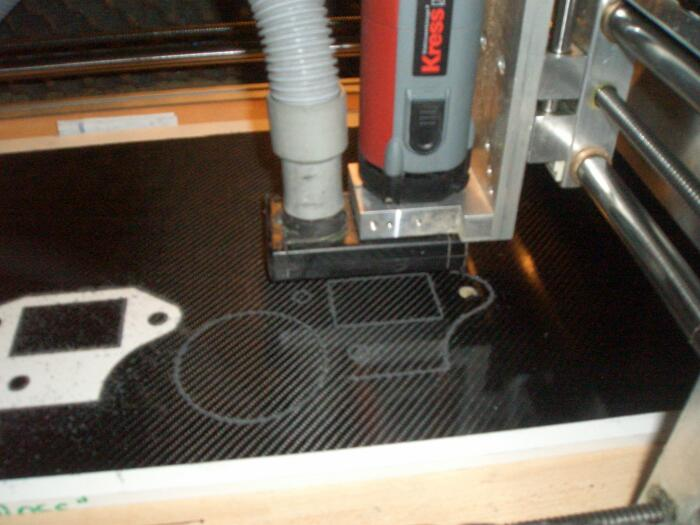
\includegraphics[width=.35\textwidth]{img/cfk.jpg}
\end{center}
\end{frame}

\begin{frame}{Square Packing}
Simple \alert{benchmark} variant:
\begin{itemize}
\item Parameter $n \in \mathbb{N}$
\item Find the minimal area to place the squares from $1$ to $n$ without overlap
\end{itemize}

\tikzset{
    task/.style={rounded corners, minimum height=3.8ex,rectangle,anchor=south west},
    task1/.style={task,draw=black, top color=isseorange!5, bottom color=isseorange!30},    
    task2/.style={task,draw=black, top color=issegrey!5, bottom color=issegrey!30},
    task3/.style={task,draw=black, top color=BrickRed!5, bottom color=BrickRed!30},
}
 
%\vspace*{-6ex}
\begin{figure}
\begin{tikzpicture}[scale=1.0,x=.5cm,y=.5cm]
    % Draw axes
    
     \node[draw, fill=issegrey!20,anchor=south west, text width=2.73cm,text height=3.73cm] at (0,0) { };  
     
    \draw [<->,thick] (0,8) node (yaxis) [above] {\texttt{height}}
        |- (6,0) node (xaxis) [right] {\texttt{width}};    

% first slide

     \node[task1,text width=.5cm,text height=.5cm] at (4.45,1) { 1 };       
     \node[task1,text width=1cm,text height=1cm] at (3.45,5.45) { 2  };   
     \node[task1,text width=2cm,text height=2cm] at (0,0) { 4  };  
     \node[task1,text width=1.5cm,text height=1.5cm] at (0,4.45) { 3 };  
     
% 
%    \node[task1,text width=1.8cm,text height=2cm] at (0,0) {  };        
%    \node[task1,text width=2.3cm,text height=.5cm] at (0,2.25) { };         
%    \node[task1,text width=2.5cm,text height=.2cm] at (2.05,0) {  }; 
%    \node[task1,text width=1.cm,text height=.2cm] at (2.05,0.6) {  };         
   
	
\end{tikzpicture}
\end{figure}

\end{frame}

\begin{frame}{Results}
\begin{center}
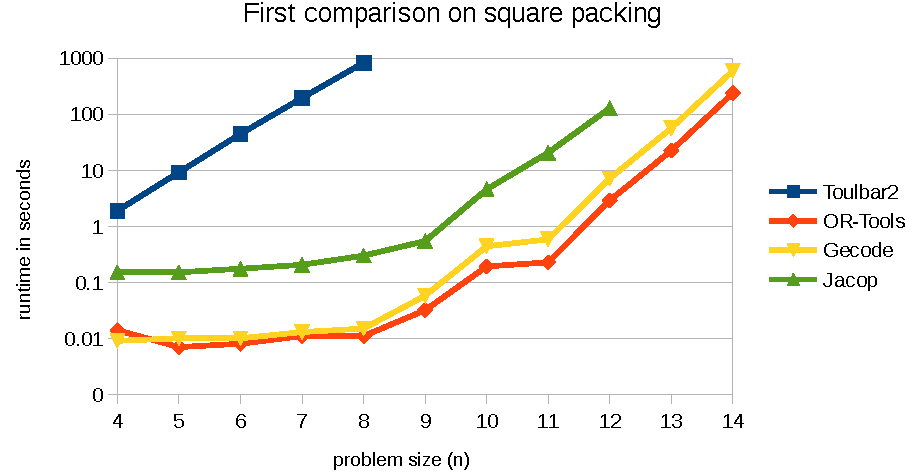
\includegraphics[width=.9\textwidth]{img/results.pdf}
\end{center}

\end{frame}
\begin{frame}{Geost}
Almost counts as a special type of ``solver'':

\begin{center}
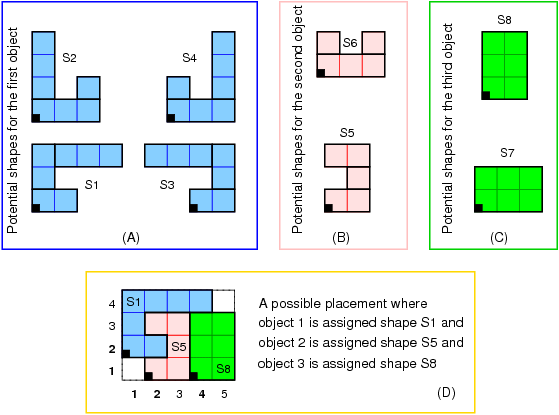
\includegraphics[width=.5\textwidth]{img/geost1.png}
\end{center}
\end{frame}

\begin{frame}{Port Scheduling}
Combines many scheduling and packing constraints:
\begin{center}
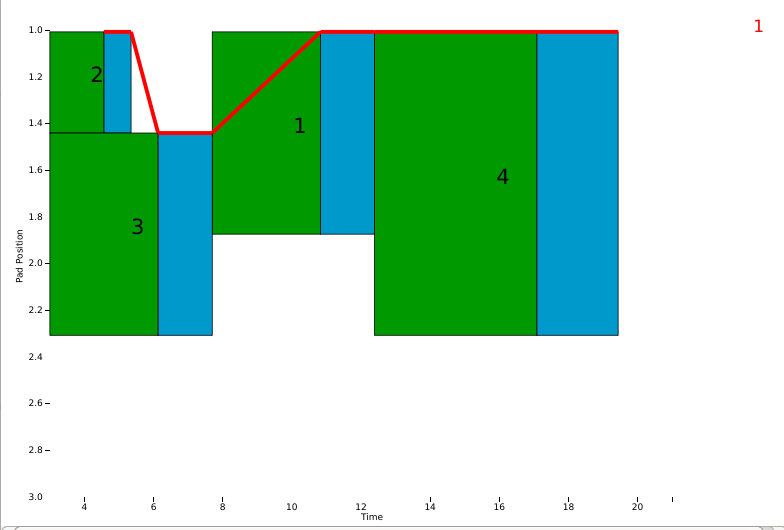
\includegraphics[width=.7\textwidth]{img/portscheduling.png}
\end{center}
\end{frame}

\begin{frame}{Scheduling: Outlook}
There's clearly much more to scheduling (that could be useful for us)
\begin{itemize}
\item Optional tasks $\rightarrow$ brings us to \alert{planning} problems
\item State-based models: Captures transitions of finite state machines~(FSM)
\item Sequence-dependent Scheduling
\begin{itemize}
\item Times for cooling down
\item Color changes 
\end{itemize} 
\end{itemize}

\begin{parchment}[Take away]
Rather easy to capture since we're dealing only with \alert{constraint models}!
\end{parchment}
\end{frame}


\begin{frame}{Soft-Constraints}

\end{frame}


\begin{frame}
\frametitle{Präferenzen im Constraint Solving}

Constraint-Problem $(X, D, C)$ 
\begin{itemize}
  \item \cemph{Variablen} $X$,
\cemph{Domänen} $D = (D_x)_{x \in X}$,
\cemph{Constraints} $C$
\end{itemize}

\vspace*{1ex}

In der Praxis: \cemph{überbestimmte} Probleme

\vspace*{2ex}

$((\{ \mathrm{x}, \mathrm{y}, \mathrm{z} \},
\mathrm{D}_{\mathrm{x}} = \mathrm{D}_{\mathrm{y}} =
\mathrm{D}_{\mathrm{z}} = \{ 1, 2, 3 \}), \{ \mathrm{c}_1,
\mathrm{c}_2, \mathrm{c}_3 \})$ mit 
\bgroup\abovedisplayskip4pt\belowdisplayskip4pt
\begin{align*}
  \mathrm{c}_1 &: \mathrm{x} + 1 = \mathrm{y}
\\[-.4ex]
  \mathrm{c}_2 &: \mathrm{z} = \mathrm{y} + 2
\\[-.4ex]
  \mathrm{c}_3 &: \mathrm{x} + \mathrm{y} \leq 3
\end{align*}
\egroup

\begin{itemize}
  \item Nicht alle Constraints können gleichzeitig erfüllt werden
\begin{itemize} \pause
  \item e.\,g., $\mathrm{c}_2$ erzwingt $\mathrm{z} = 3$ und $\mathrm{y} = 1$, im Konflikt mit $\mathrm{c}_1$
\end{itemize}

  \item Ein Agent \cemph{wählt} zwischen Zuweisungen, die $\{ \mathrm{c}_1, \mathrm{c}_3 \}$ oder $\{ \mathrm{c}_2, \mathrm{c}_3 \}$ erfüllen.
\end{itemize}

\vspace*{2ex}

Welche Zuweisungen $v \in [X \to D]$ sollen \alert{bevorzugt} werden von einem Agenten (oder sogar einer Menge von Agenten)?

\end{frame}

\begin{frame}
\frametitle{Constraint Relationships}

Ansatz~\cite{Schiendorfer13}
\begin{itemize}
  \item Definiere Relation $R$ über Constraints $C$ um anzugeben, welche Constraints wichtiger sind als andere, e.\,g.
\begin{itemize}
  \item $\mathrm{c}_1$ wichtiger als $\mathrm{c}_2$

  \item $\mathrm{c}_1$ wichtiger als $\mathrm{c}_3$
\end{itemize}
\end{itemize}
\begin{textblock*}{2.5cm}[1,1](\textwidth-1.5cm,\textheight-4.03cm)
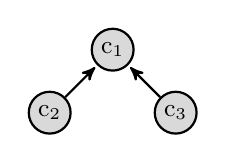
\begin{tikzpicture}[auto,
                    ->,>=stealth',shorten >=1pt,thick,
                    node distance=.7cm,inner sep=2pt,
                    constraint/.style={circle,fill=black!15,draw,font=\sffamily\small}]
\node[constraint node] (1) at (0, 0)                   {$\mathrm{c}_1$};
\node[constraint node] (2) at ($ (1) + (-0.8, -0.8) $) {$\mathrm{c}_2$};  
\node[constraint node] (3) at ($ (1) + ( 0.8, -0.8) $) {$\mathrm{c}_3$};  
%  
\path[every node/.style={font=\sffamily\tiny}]
  (2) edge (1)
  (3) edge (1)
  ;
\end{tikzpicture}
\end{textblock*}

\vspace*{5.6ex}

Benefits
\begin{itemize}
  \item \cemph{Qualitativer} Formalismus --- einfach zu spezifizieren
\begin{itemize}
 \item Hebe diese Relation auf Verletzungsmengen
  \item \cemph{Dominanzeigenschaften} regulieren den Tradeoff ``Hierarchie vs. Egalitär''
  \item Single-Predecessors-Dominance (SPD) vs. Transitive-Predecessors-Dominance (TPD)
\end{itemize}

\end{itemize}

%\vspace*{2ex}
%\begin{small}
%A.~Schiendorfer, J.-Ph.~Steghöfer, A.~Knapp, F.~Nafz, W.~Reif (2013)
%\end{small}
\end{frame}

\begin{frame}[fragile]{MiniBrass}

\begin{center}


\includegraphics[width=.5\textwidth]{img/minibrass.png}

\vspace*{2ex}

\url{http://isse-augsburg.github.io/constraint-relationships/}

\end{center}

\end{frame}

\begin{frame}
\frametitle{Single-Predecessor-Dominance (SPD) Lifting}

\cemph{isWorseThan}-Relation für Mengen verletzter Constraints
%
%\bgroup\abovedisplayskip=4pt\belowdisplayskip=12pt
%\begin{gather*}
%  V \SPDrel{R} V \uplus \{ c \} 
%\\
%  V \uplus \{ c \} \SPDrel{R} V \uplus \{ c' \}
%\quad\text{if $c \rightarrow_R c'$}
%\end{gather*}
%\egroup

\begin{center}
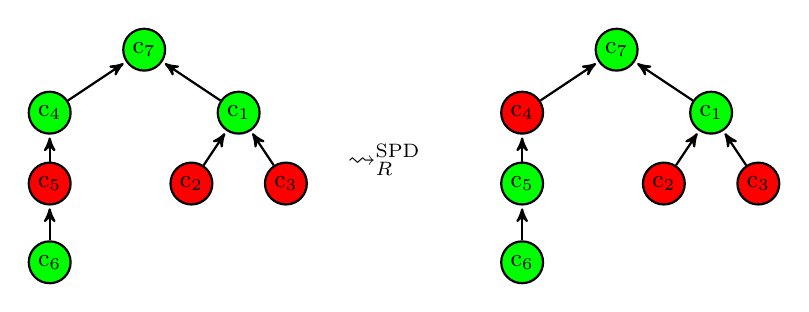
\begin{tikzpicture}[auto,
                    ->,>=stealth',shorten >=1pt,thick,
                    node distance=1cm,inner sep=2pt,
                    constraint/.style={circle,fill=black!15,draw,font=\sffamily\small}]
\begin{scope}
\node[constraint,fill=green] (1) at (0, 0)                   {$\mathrm{c}_7$};
\node[constraint,fill=green] (2) at ($ (1) + (-1.2, -0.8) $) {$\mathrm{c}_4$};  
\node[constraint,fill=red]   (3) at ($ (2) + (0.0, -0.9) $) {$\mathrm{c}_5$};  
\node[constraint,fill=green] (4) at ($ (3) + ( 0.0, -1.0) $) {$\mathrm{c}_6$};
\node[constraint,fill=green] (7) at ($ (1) + ( 1.2, -0.8) $) {$\mathrm{c}_1$};  
\node[constraint,fill=red]   (8) at ($ (7) + (-0.6, -0.9) $) {$\mathrm{c}_2$};  
\node[constraint,fill=red]   (9) at ($ (7) + ( 0.6, -0.9) $) {$\mathrm{c}_3$};  
%  
\path[every node/.style={font=\sffamily\tiny}]
  (2) edge (1)
  (7) edge (1)
  (3) edge (2)
  (4) edge (3)
  (8) edge (7)
  (9) edge (7)
  ;
\end{scope}
%
\begin{scope}[xshift=6cm]
\node[constraint,fill=green] (1) at (0, 0)                   {$\mathrm{c}_7$};
\node[constraint,fill=red]   (2) at ($ (1) + (-1.2, -0.8) $) {$\mathrm{c}_4$};  
\node[constraint,fill=green] (3) at ($ (2) + (0.0, -0.9) $) {$\mathrm{c}_5$};  
\node[constraint,fill=green] (4) at ($ (3) + ( 0.0, -1.0) $) {$\mathrm{c}_6$};  
\node[constraint,fill=green] (7) at ($ (1) + ( 1.2, -0.8) $) {$\mathrm{c}_1$};  
\node[constraint,fill=red]   (8) at ($ (7) + (-0.6, -0.9) $) {$\mathrm{c}_2$};  
\node[constraint,fill=red]   (9) at ($ (7) + ( 0.6, -0.9) $) {$\mathrm{c}_3$};  
%  
\path[every node/.style={font=\sffamily\tiny}]
  (2) edge (1)
  (7) edge (1)
  (3) edge (2)
  (4) edge (3)
  (8) edge (7)
  (9) edge (7)
  ;
\end{scope}
%
\node (R) at (3.05, -1.4) {$\SPDrel{R}$};
\end{tikzpicture}
\end{center}
%
%\cemph{Ordnungs}relation über Zuweisungen 
%\bgroup\abovedisplayskip4pt
%\begin{equation*}
%  w \SPDord{R} v \iff \{ c \in C \mid v \not\models c \} \mathrel{({\SPDrel{R}})^{+}} \{ c \in C \mid w \not\models c \}
%\end{equation*}
%\egroup

\end{frame}


\begin{frame}
\frametitle{Transitive-Predecessors-Dominance (TPD) Lifting}

\cemph{isWorseThan}-Relation für Mengen verletzter Constraints
%
%\bgroup\abovedisplayskip=4pt\belowdisplayskip=12pt
%\begin{gather*}
%  V \TPDrel{R} V \uplus \{ c \} 
%\\
%  V \uplus \{ c_1, \ldots, c_k \} \TPDrel{R} V \uplus \{ c' \}
%\quad\text{if $\forall c \in \{ c_1, \ldots, c_k \} \,.\, c \rightarrow_{R}^{+} c'$}
%\end{gather*}
%\egroup

\begin{center}
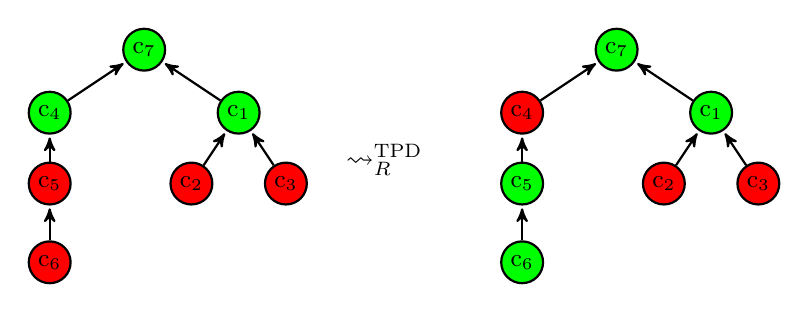
\begin{tikzpicture}[auto,
                    ->,>=stealth',shorten >=1pt,thick,
                    node distance=1cm,inner sep=2pt,
                    constraint/.style={circle,fill=black!15,draw,font=\sffamily\small}]
\begin{scope}
\node[constraint,fill=green] (1) at (0, 0)                   {$\mathrm{c}_7$};
\node[constraint,fill=green] (2) at ($ (1) + (-1.2, -0.8) $) {$\mathrm{c}_4$};  
\node[constraint,fill=red]   (3) at ($ (2) + (0.0, -0.9) $) {$\mathrm{c}_5$};  
\node[constraint,fill=red] (4) at ($ (3) + ( 0.0, -1.0) $) {$\mathrm{c}_6$};
\node[constraint,fill=green] (7) at ($ (1) + ( 1.2, -0.8) $) {$\mathrm{c}_1$};  
\node[constraint,fill=red]   (8) at ($ (7) + (-0.6, -0.9) $) {$\mathrm{c}_2$};  
\node[constraint,fill=red]   (9) at ($ (7) + ( 0.6, -0.9) $) {$\mathrm{c}_3$};  
%  
\path[every node/.style={font=\sffamily\tiny}]
  (2) edge (1)
  (7) edge (1)
  (3) edge (2)
  (4) edge (3)
  (8) edge (7)
  (9) edge (7)
  ;
\end{scope}
%
\begin{scope}[xshift=6cm]
\node[constraint,fill=green] (1) at (0, 0)                   {$\mathrm{c}_7$};
\node[constraint,fill=red]   (2) at ($ (1) + (-1.2, -0.8) $) {$\mathrm{c}_4$};  
\node[constraint,fill=green] (3) at ($ (2) + (0.0, -0.9) $) {$\mathrm{c}_5$};  
\node[constraint,fill=green] (4) at ($ (3) + ( 0.0, -1.0) $) {$\mathrm{c}_6$};  
\node[constraint,fill=green] (7) at ($ (1) + ( 1.2, -0.8) $) {$\mathrm{c}_1$};  
\node[constraint,fill=red]   (8) at ($ (7) + (-0.6, -0.9) $) {$\mathrm{c}_2$};  
\node[constraint,fill=red]   (9) at ($ (7) + ( 0.6, -0.9) $) {$\mathrm{c}_3$};  
%  
\path[every node/.style={font=\sffamily\tiny}]
  (2) edge (1)
  (7) edge (1)
  (3) edge (2)
  (4) edge (3)
  (8) edge (7)
  (9) edge (7)
  ;
\end{scope}
%
\node (R) at (3.05, -1.4) {$\TPDrel{R}$};
\end{tikzpicture}
\end{center}

%\cemph{Ordnungs}relation über Zuweisungen
%\bgroup\abovedisplayskip4pt
%\begin{equation*}
%  w \TPDord{R} v \iff \{ c \in C \mid v \not\models c \} \mathrel{({\TPDrel{R}})^{+}} \{ c \in C \mid w \not\models c \}
%\end{equation*}
%\egroup

\end{frame}

% block styles
\tikzstyle{sensor}=[draw, fill=blue!20, text width=5em, 
    text centered, minimum height=2.5em,drop shadow]    
    
\tikzstyle{alg} = [sensor, text width=5em, fill=isseorange!20, 
    minimum height=13em, rounded corners, drop shadow]
\tikzstyle{constraint}=[draw, circle, fill=issegrey!20, text width=1.2em, 
    text centered, minimum height=1.5em,drop shadow]
\tikzstyle{domainstore} = [alg, text width=5em, fill=isseorange!40, 
    minimum height=4em, rounded corners]
\tikzstyle{goodc} = [ForestGreen, font=\bfseries]
\tikzstyle{badc} = [Red, font=\bfseries]
\tikzstyle{okayc} = [LimeGreen, font=\bfseries]
        
\tikzset{
vecArrow/.style={
  thick
  }
}

\tikzset{
    mn/.style={rectangle,rounded corners,draw=black, top color=isseorange!5, bottom color=isseorange!30,
                   very thick, inner sep=\myinnersep*1em, minimum size=3em, text centered, outer sep=0, align=center},
    innernode/.style={mn, text width=3cm,  minimum height=1.5cm,
                      top color=issegrey!20, bottom color=issegrey!60},
    emphnode/.style={innernode, top color=isseorange!30, bottom color=isseorange!70}
}

% Define distances for bordering
\def\blockdist{2.3}
\def\edgedist{2.5}

  \tikzset{
    invisible/.style={opacity=0},
    visible on/.style={alt={#1{}{invisible}}},
    alt/.code args={<#1>#2#3}{%
      \alt<#1>{\pgfkeysalso{#2}}{\pgfkeysalso{#3}} % \pgfkeysalso doesn't change the path
    },
  }
  
\begin{frame}{Traditional Constraint Solving}
\begin{center}
\begin{tikzpicture}
% First row:
 \node (search) [alg]  {Search \phantom{$x = 5$} };
 \path (search.east)+(4.6,0) node (propag) [alg,text width =12em]  {};
 \node[below right] at (propag.north west) {Constraint Store $C$};
 
 \path (propag.west)+(0.8,-1.2) node (c1) [constraint] {$c_1$}; 
 \path (propag.west)+(1.1,-0.2) node (c2) [constraint] {$c_2$}; 
 \path (propag.west)+(2.0,0.4) node (c3) [constraint] {$c_3$}; 
 \path (propag.west)+(3.2,0.7) node (c4) [constraint] {$c_4$};
  
 \path (propag.east)+(-1.2,-1.2) node (domainstore) [domainstore] {Domain Store $(D_x)_{x \in X}$}; 
 
 \path [draw,vecArrow, ->] ([yshift=-2em]search.north east) -- node [above,visible on=<2->] {$x\gets5$} ([yshift=-2em]propag.north west);
 \path [draw,vecArrow, <-] ([yshift=2em]search.south east) -- node [above,goodc,visible on=<4->] {$\top$} ([yshift=2em]propag.south west);
 
 \path [draw, vecArrow, <->] (c1.east) -- node [below,visible on=<3->,goodc] {$\top$} (domainstore.west) ;
 \path [draw,vecArrow, <->] (c2.330) -- node [above right,visible on=<3->,goodc] {$\top$} (domainstore.150) ;
 \path [draw,vecArrow, <->] (c3.290) -- node [right,visible on=<3->,goodc] {$\top$} (domainstore.120) ;
 \path [draw,vecArrow, <->] (c4.south) -- node [right,visible on=<3->,goodc] {$\top$} (domainstore.68) ;
\end{tikzpicture}
\end{center}
\onslide<0>{
\begin{columns}[c] % contents are top vertically aligned
     \begin{column}[c]{7cm} % each column can also be its own 
\begin{itemize}
\item Eine Menge von Erfüllungsgraden, $\mathbb{B} = \{ \bot, \top \}$
\item Eine Kombinationsoperation $\wedge$
\item Ein neutrales Element $\top$
\item Eine partielle Ordnung $(\mathbb{B}, \leq_\mathbb{B})$ mit $\top <_\mathbb{B} \bot$ 
\end{itemize}
\end{column}
     \begin{column}[c]{4.5cm} 
     \end{column} 
\end{columns}
}

\end{frame}

\begin{frame}{Klassisches Constraint-Solving}
\begin{center}
\begin{tikzpicture}
% First row:
 \node (search) [alg]  {Search $x = 5$};
 \path (search.east)+(4.6,0) node (propag) [alg,text width =12em]  {};
 \node[below right] at (propag.north west) {Constraint Store $C$};
 
 \path (propag.west)+(0.8,-1.2) node (c1) [constraint] {$c_1$}; 
 \path (propag.west)+(1.1,-0.2) node (c2) [constraint] {$c_2$}; 
 \path (propag.west)+(2.0,0.4) node (c3) [constraint] {$c_3$}; 
 \path (propag.west)+(3.2,0.7) node (c4) [constraint] {$c_4$};
  
 \path (propag.east)+(-1.2,-1.2) node (domainstore) [domainstore] {Domain Store $(D_x)_{x \in X}$}; 
 
 \path [draw,vecArrow, ->] ([yshift=-2em]search.north east) -- node [above,visible on=<2->] {$y \gets 4$} ([yshift=-2em]propag.north west);
 \path [draw,vecArrow, <-] ([yshift=2em]search.south east) -- node [below,badc,visible on=<4->] {$\bot$} ([yshift=2em]propag.south west);
 
 \path [draw, vecArrow, <->] (c1.east) -- node [below,visible on=<3->,badc] {$\bot$} (domainstore.west) ;
 \path [draw,vecArrow, <->] (c2.330) -- node [above right,visible on=<3->,goodc] {$\top$} (domainstore.150) ;
 \path [draw,vecArrow, <->] (c3.290) -- node [right,visible on=<3->,goodc] {$\top$} (domainstore.120) ;
 \path [draw,vecArrow, <->] (c4.south) -- node [right,visible on=<3->,goodc] {$\top$} (domainstore.68) ;
\end{tikzpicture}
\end{center}
\onslide<5->{
\begin{columns}[c] % contents are top vertically aligned
     \begin{column}[c]{7cm} % each column can also be its own 
\begin{itemize}
\item Eine Menge von Erfüllungsgraden, $\mathbb{B} = \{ \bot, \top \}$
\item Eine Kombinationsoperation $\wedge$
\item Ein neutrales Element $\top$
\item Eine partielle Ordnung $(\mathbb{B}, \leq_\mathbb{B})$ mit $\top <_\mathbb{B} \bot$ 
\end{itemize}
   \end{column} 
     \begin{column}[c]{4.5cm} 
     \end{column} 
\end{columns}
}
\end{frame}

\begin{frame}{Soft-Constraint-Solving}
\begin{center}
\begin{tikzpicture}
% First row:
 \node (search) [alg]  {Search $x = 5$};
 \path (search.east)+(4.6,0) node (propag) [alg,text width =12em]  {};
 \node[below right] at (propag.north west) {Constraint Store $C$};
 
 \path (propag.west)+(0.8,-1.2) node (c1) [constraint] {$c_1$}; 
 \path (propag.west)+(1.1,-0.2) node (c2) [constraint] {$c_2$}; 
 \path (propag.west)+(2.0,0.4) node (c3) [constraint] {$c_3$}; 
 \path (propag.west)+(3.2,0.7) node (c4) [constraint] {$c_4$};
  
 \path (propag.east)+(-1.2,-1.2) node (domainstore) [domainstore] {Domain Store $(D_x)_{x \in X}$}; 
 
 \path [draw,vecArrow, ->] ([yshift=-2em]search.north east) -- node [above,visible on=<2->] {$y \gets 4$} ([yshift=-2em]propag.north west);
 \path [draw,vecArrow, <-] ([yshift=2em]search.south east) -- node [below,okayc,visible on=<4->] {$4$} ([yshift=2em]propag.south west);
 
 \path [draw, vecArrow, <->] (c1.east) -- node [below,visible on=<3->,okayc] {$4$} (domainstore.west) ;
 \path [draw,vecArrow, <->] (c2.330) -- node [above right,visible on=<3->,goodc] {$0$} (domainstore.150) ;
 \path [draw,vecArrow, <->] (c3.290) -- node [right,visible on=<3->,goodc] {$0$} (domainstore.120) ;
 \path [draw,vecArrow, <->] (c4.south) -- node [right,visible on=<3->,goodc] {$0$} (domainstore.68) ;
\end{tikzpicture}
\end{center}
\onslide<5->{
\begin{columns}[c] % contents are top vertically aligned
     \begin{column}[c]{7cm} % each column can also be its own environment
    \begin{itemize}
\item Eine Menge von Erfüllungsgraden, e.g., $\{ 0, \ldots, k \}$
\item Eine Kombinationsoperation $+$
\item Ein neutrales Element $0$
\item Eine partielle Ordnung $(\mathbb{N}, \geq)$ mit $0$ als Top 
\end{itemize}
   \end{column} \pause
     \begin{column}[c]{4.5cm} 
    %    Eine \cemph{valuation structure}~\cite{Schiex1995valued}, wenn die Ordnung total ist, sonst eine  \cemph{partial valuation structure}~\cite{Gadducci2013} (PVS).
     \end{column}
\end{columns}
    
}
\end{frame}

\begin{frame}[fragile]{SoftConstraints in MiniZinc}
\begin{lstlisting}
% X: {x,y,z} D_i = {1,2,3}, i in X
%    * c1: x + 1 = y   * c2: z = y + 2 * c3: x + y <= 3
% (c) ISSE
% isse.uni-augsburg.de/en/software/constraint-relationships/
include "soft_constraints/minizinc_bundle.mzn";

var 1..3: x; var 1..3: y; var 1..3: z;

% read as "soft constraint c1 is satisfied iff x + 1 = y"
constraint x + 1 = y <-> satisfied[1];
constraint z = y + 2 <-> satisfied[2];
constraint x + y <= 3 <-> satisfied[3];

% soft constraint specific for this model
nScs = 3; nCrEdges = 2;
crEdges = [| 2, 1 | 3, 1 |]; % read c2 is less important than c1

solve minimize penSum; % minimize the sum of penalties
\end{lstlisting}

\end{frame}

\begin{frame}[fragile]{Search types}
The whole valuation space (partially ordered)

\begin{figure}[!t]
\begin{center}
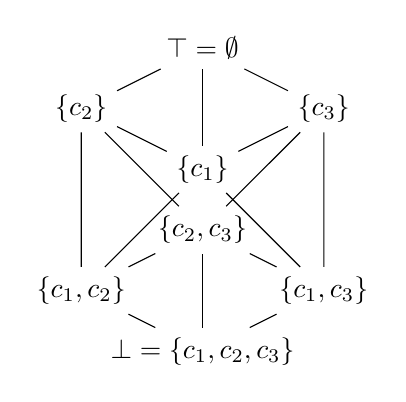
\begin{tikzpicture}[scale=0.77,auto]

% single PVS
\node (bot) at (0,0) {$\bot = \{c_1, c_2, c_3 \}$};
\node (c1c2) at (-2,1) {$\{c_1, c_2\}$};
\node (c2c3) at (0,2) {$\{c_2, c_3\}$};
\node (c1c3) at (2,1) {$\{c_1, c_3\}$};

\node (c1) at (0,3) {$\{c_1\}$};
\node (c2) at (-2,4) {$\{c_2\}$};
\node (c3) at (2,4) {$\{c_3\}$};
%\node (a) at (-1,0.5) {$a$};
%\node (b) at (-1,1.5) {$b$};
%\node (c) at (1,1) {$c$};
\node (top) at (0,5) {$\top = \emptyset$};


\path[-]
(bot) edge (c1c2)
      edge (c2c3)
      edge (c1c3)
(c1c2) edge (c2c3)
(c1c3) edge (c2c3)
(c1c3) edge (c1)
(c1c3) edge (c3)
(c2c3) edge (c2)
(c2c3) edge (c3)
(c1c2) edge (c1)
(c1c2) edge (c2)
(c1) edge (c2)
(c1) edge (c3)
(c2) edge (top)
(c1) edge (top)
(c3) edge (top)
      ;
%(a) edge (b)
%(b) edge (top)
%(bot) edge (c)
%(c) edge (top)
;

\end{tikzpicture}
\end{center}
\label{fig:nosuprema}
\end{figure}
%\onslide<0>{
\begin{lstlisting}
%
% Typical Optimization Routine (Branch and Bound):
%
%  1. Look for the first feasible solution
%  2. Impose restrictions on the next feasible solution
%  3. Repeat
\end{lstlisting}
%}
\end{frame}


\tikzset{onslide/.code args={<#1>#2}{%
  \only<#1>{\pgfkeysalso{#2}}
}}
\tikzstyle{highlight}=[isseorange,ultra thick]
\tikzstyle{highlight2}=[CornflowerBlue,ultra thick]

\begin{frame}[fragile]{Search types: Strictly better}
The whole valuation space (partially ordered)



\begin{figure}[!t]
\begin{center}
\begin{tikzpicture}[scale=0.77,auto]

% single PVS
\node (bot) at (0,0) {\alert{$\bot = \{c_1, c_2, c_3 \}$}};
\node (c1c2) at (-2,1) {\alert<2->{$\{c_1, c_2\}$}};
\node (c2c3) at (0,2) {$\{c_2, c_3\}$};
\node (c1c3) at (2,1) {$\{c_1, c_3\}$};

\node (c1) at (0,3) {\alert<3->{$\{c_1\}$}};
\node (c2) at (-2,4) {\alert<4->{$\{c_2\}$}};
\node (c3) at (2,4) {$\{c_3\}$};
%\node (a) at (-1,0.5) {$a$};
%\node (b) at (-1,1.5) {$b$};
%\node (c) at (1,1) {$c$};
\node (top) at (0,5) {$\top = \emptyset$};


\path[-]
(bot) edge[onslide={<2->{highlight}}] (c1c2)
      edge (c2c3)
      edge (c1c3)
(c1c2) edge (c2c3)
(c1c3) edge (c2c3)
(c1c3) edge (c1)
(c1c3) edge (c3)
(c2c3) edge (c2)
(c2c3) edge (c3)
(c1c2) edge[onslide={<3->{highlight}}] (c1)
(c1c2) edge (c2)
(c1) edge[onslide={<4->{highlight}}] (c2)
(c1) edge (c3)
(c2) edge (top)
(c1) edge (top)
(c3) edge (top)
      ;
%(a) edge (b)
%(b) edge (top)
%(bot) edge (c)
%(c) edge (top)
;

\end{tikzpicture}
\end{center}
\label{fig:nosuprema}
\end{figure}
\begin{lstlisting}
function ann: strictlyBetterBAB(var set of SOFTCONSTRAINTS: vScs) 
      = repeat(
           if next() then 
             commit() /\ 
             post(isWorse(sol(vScs), vScs))
           else break endif       );
\end{lstlisting}
\end{frame}

\begin{frame}[fragile]{Search types: Only not dominated}
The whole valuation space (partially ordered)

\begin{figure}[!t]
\begin{center}
\begin{tikzpicture}[scale=0.77,auto]

% single PVS
\node (bot) at (0,0) {\alert{$\bot = \{c_1, c_2, c_3 \}$}};
\node (c1c2) at (-2,1) {\alert<2->{$\{c_1, c_2\}$}};
\node[onslide={<4->{highlight2}}] (c2c3) at (0,2) {$\{c_2, c_3\}$};
\node (c1c3) at (2,1) {$\{c_1, c_3\}$};

\node (c1) at (0,3) {\alert<3->{$\{c_1\}$}};
\node (c2) at (-2,4) {\alert<5->{$\{c_2\}$}};
\node [onslide={<6->{highlight2}}](c3) at (2,4) {$\{c_3\}$};
%\node (a) at (-1,0.5) {$a$};
%\node (b) at (-1,1.5) {$b$};
%\node (c) at (1,1) {$c$};
\node (top) at (0,5) {$\top = \emptyset$};


\path[-]
(bot) edge[onslide={<2->{highlight}}] (c1c2)
      edge (c2c3)
      edge (c1c3)
(c1c2) edge[onslide={<4->{highlight2}}] (c2c3)
(c1c3) edge (c2c3)
(c1c3) edge (c1)
(c1c3) edge (c3)
(c2c3) edge (c2)
(c2c3) edge[onslide={<6->{highlight2}}] (c3)
(c1c2) edge[onslide={<3->{highlight}}] (c1)
(c1c2) edge (c2)
(c1) edge[onslide={<5->{highlight}}] (c2)
(c1) edge (c3)
(c2) edge (top)
(c1) edge (top)
(c3) edge (top)
      ;

\end{tikzpicture}
\end{center}
\label{fig:nosuprema}
\end{figure}
\begin{lstlisting}
function ann: strictlyBetterBAB(var set of SOFTCONSTRAINTS: vScs) 
      = repeat(
           if next() then 
             commit() /\ 
             post((isWorse(vScs, sol(vScs)) \/ vScs = sol(vScs)))
           else break endif       );
\end{lstlisting}
\end{frame}




\begin{frame}{Case Studies}
Applied to domains where 
\begin{itemize}
\item Certain properties should really capture \alert{preferences}, not constraints
\item at design time, it is \alert{unclear} whether an instance is actually solvable
\item Solution space is \emph{combinatorial}
\begin{itemize}
\item[-] Discrete choices
\item[-] Additional hard constraints
\end{itemize}
\end{itemize}

\vspace*{2ex}

Illustrative case studies (found in \texttt{example-problems})
\begin{itemize}
\item Mentor Matching
\item Exam Scheduling
\item Power Plant Scheduling
\end{itemize}
\end{frame}


\begin{frame}[fragile]{Mentor Matching}

\textbf{Goal}: Assign mentees (e.g. students) to mentors (e.g. companies) such that 
\begin{itemize}
\item Students are most satisfied with their mentors 
\item Companies are satisfied with their mentees
\item Two-sided preferences
\end{itemize}

\vspace*{2ex}

So far, sounds like a typical \emph{stable matching} problem, but:

\begin{itemize}
\item We do not have a 1:1 mapping (companies advise several students)
\item Additional constraints are present
\begin{itemize}
\item[-] Each company has to advise at least $l$, at most $u$ students
\item[-] The number of advised students \emph{should} be roughly equal per company (fairness)
\item[-] Students actually despising a company should not be forced to go there (\emph{hard exclusion} of solutions)
\end{itemize}
\end{itemize}
\end{frame}


\begin{frame}[fragile]{Mentor Matching: Example}
\begin{center}
\tikzset{onslide/.code args={<#1>#2}{%
  \only<#1>{\pgfkeysalso{#2}}
}}

\tikzstyle{highlight}=[isseorange,ultra thick]
\tikzstyle{highlight2}=[CornflowerBlue,ultra thick,rounded corners]
\tikzstyle{defaultStyle}=[white,ultra thick,rounded corners]

\tikzstyle{impo}=[dashed]
\begin{tikzpicture}[every node/.style={
anchor=base,
%text depth=.5ex,
%text height=2ex,
%minimum height=2ex,
align=center,
rectangle,
text width=2em
}]
\matrix (magic) [nodes in empty cells, ampersand replacement=\&,row sep=0.4cm,column sep=1.5cm]
{
\node[draw,defaultStyle, onslide={<3->{highlight2}}](s1){
\includegraphics[width=\textwidth]{img/businessman.png}}; \& \& \& \node[text width=4em, defaultStyle, draw, onslide={<3->{highlight2}}](c1) {
\includegraphics[width=\textwidth]{img/airplane.png}}; \\
\node(s2){
\includegraphics[width=\textwidth]{img/woman.png}};       \& \& \& \node(c2) {
\includegraphics[width=2\textwidth]{img/logistics.png}}; \\
\node(s3){
\includegraphics[width=\textwidth]{img/man.png}};         \& \& \& \node(c3) {
\includegraphics[width=2\textwidth]{img/enrgy.png}}; \\
\node[defaultStyle, draw, onslide={<3->{highlight2}}](s4){
\includegraphics[width=\textwidth]{img/woman2.png}};      \& \\
};

\draw[onslide={<2->{highlight}}] (s1) -- (c1);
\draw[] (s1) -- (c2);

\draw[onslide={<2->{highlight}}] (s2) -- (c1);
\draw[] (s2) -- (c3);

\draw[onslide={<2->{highlight}}] (s3) -- (c2);

\draw[onslide={<2->{highlight}}] (s4) -- (c3);
\draw[] (s4) -- (c2);
%
%\draw[onslide={<1-2>{highlight}}] (z) -- (3);
%\draw[onslide={<3>{highlight}}] (z) -- (2);
%
%\draw[onslide={<1-2>{highlight}}] (t) -- (2);
%\draw[] (t) -- (1);
%\draw[onslide={<3>{highlight}}] (t) -- (5);
%\draw[] (t) -- (3);
%\draw[] (t) -- (4);
%\draw[onslide={<1>{highlight}}] (u) -- (4);
%\draw[] (u) -- (3);
%\draw[] (u) -- (5);
%\draw[] (u) -- (6);
\end{tikzpicture}
\end{center}
\onslide<2->{This \alert{assignment} respects the students' preferences (edges) \onslide<3->{but ignores the {\color{CornflowerBlue} companies' preferences}.}}
\onslide<4->{\tiny ok, it's not really a \emph{matching} since companies supervise more than one student \ldots }
\end{frame}

\begin{frame}[fragile]{Mentor Matching: Model}
\begin{lstlisting}
int: n; set of int: STUDENT = 1..n;
int: m; set of int: COMPANY = 1..m;

% assign students to companies
array[STUDENT] of var COMPANY: worksAt;

% insert relationships of students and companies here

int: minPerCompany = 2; int: maxPerCompany = 3;
constraint global_cardinality_low_up ( 
           worksAt, [c | c in COMPANY], 
           [minPerCompany | c in COMPANY], 
           [maxPerCompany | c in COMPANY]); 
           
solve 
:: int_search([ satisfied[mostImpFirst[i]] | i in SOFTCONSTRAINTS], 
  input_order, indomain_max, complete)
minimize penSum;
\end{lstlisting}
\end{frame}

\begin{frame}[fragile]{Mentor Matching: Preferences}
\begin{lstlisting}
n = 3; m = 3;
int: brenner = 1;
int: teufel = 2;
int: fennek  = 3;

int: cupgainini = 1;
int: gsm = 2;
int: junedied = 3;

% specify soft constraints, order by relationship
constraint worksAt[teufel] = junedied <-> satisfied[teufJune];
constraint worksAt[teufel] = cupgainini <-> satisfied[teufCap];
constraint worksAt[teufel] = gsm <-> satisfied[teufGsm];

constraint worksAt[fennek ] in {cupgainini, gsm}  <-> satisfied[fenFavs];
constraint worksAt[fennek ] in {junedied} <-> satisfied[fenOK];

crEdges = [| teufGsm, teufCap | teufGsm, teufJune 
            | fenOK, fenFavs |];
\end{lstlisting}
\end{frame}

\begin{frame}[fragile]{Mentor Matching: Refinements}
Split company and student preferences:
\begin{lstlisting}
% first, our students' preferences
var int: penStud = sum(sc in 1..lastStudentPref) 
     (bool2int(not satisfied[sc]) * penalties[sc]);
% now companies' preferences
var int: penComp = sum(sc in lastStudentPref+1..nScs)
     (bool2int(not satisfied[sc]) * penalties[sc]);
\end{lstlisting}

\vspace*{3ex}

Optimize lexicographically

\begin{lstlisting}
solve 
:: int_search([ satisfied[mostImpFirst[i]] | i in SOFTCONSTRAINTS],%... 
%search minimize_lex([penStud, penComp]) /\ if % ...
search minimize_lex([penComp, penStud]) /\ if % ...
\end{lstlisting}
\end{frame}

\begin{frame}[fragile]{Mentor Matching: Priority Example}
Taken from example: \texttt{student-company-matching.mzn}
\begin{lstlisting}
solve 
:: int_search([ satisfied[mostImpFirst[i]] | i in SOFTCONSTRAINTS],%... 
search minimize_lex([penStud, penComp]) /\ if %...
\end{lstlisting}

\small
\begin{verbatim}
worksAt = [1, 3, 2, 3], penalty Students: 8, penalty Companies: 6
----------
==========
\end{verbatim}

\begin{lstlisting}
solve 
:: int_search([ satisfied[mostImpFirst[i]] | i in SOFTCONSTRAINTS],%... 
search minimize_lex([penStud, penComp]) /\ if %...
\end{lstlisting}

\small
\begin{verbatim}
worksAt = [1, 3, 1, 2], penalty Students: 10, penalty Companies: 4
----------
==========
\end{verbatim}
Here, company 1 (cupgainini) wanted to have student 3, and company 2 (APS) did not have any preferences whatsoever (so accepted student 4 instead of 3). Student 4 would have liked company 3 (junedied) better, though.
\end{frame}

\begin{frame}[fragile]{Mentor Matching: Real Instance}
\begin{itemize}
\item Collected data from winter term

\begin{parchment}
\begin{verbatim}
"the favorites":
1. JuneDied-Lynx- HumanIT
2. Cupgainini
 
"I could live with that":
3. Seamless-German
4. gsm systems
5. Yiehlke
 
"I think, we won't be happy":
6. APS
7. Delphi Databases
\end{verbatim} 
\end{parchment}
\end{itemize}
\end{frame}

\begin{frame}[fragile]{Mentor Matching: Real Instance}
\begin{itemize}
\item Gave precedence to \alert{students}
\begin{itemize}
\item[-] After all, what should companies do with unhappy students?
\end{itemize}
\item Search space: 7 companies for 16 students $\rightarrow 7^{16} = 3.3233 \cdot 10^{13}$
\vspace*{2ex}
\item Led to a constraint problem with 
\begin{itemize}
\item[-] 77 student preferences (soft constraints) from 16 students
\item[-] of a total of 114 soft constraints (37 company preferences) 
\end{itemize}

\vspace*{2ex}

\item \emph{Proved} optimal solution 
\begin{itemize}
\item[-] 4 minutes compilation 
\item[-] another 2m 12s solving time
\end{itemize}
\end{itemize}
\end{frame}


\begin{frame}[fragile]{Exam Scheduling}

\textbf{Goal}: Assign exam dates to students such that 
\begin{itemize}
\item Each student likes their appoints (\emph{approves of it})
\item The number of distinct dates is minimized (to reduce time investment of teachers)
\end{itemize}

%\vspace*{2ex}
%\begin{parchment}
\begin{center}

\includegraphics[width=.15\textwidth]{img/voting.png}
\hspace*{4ex}
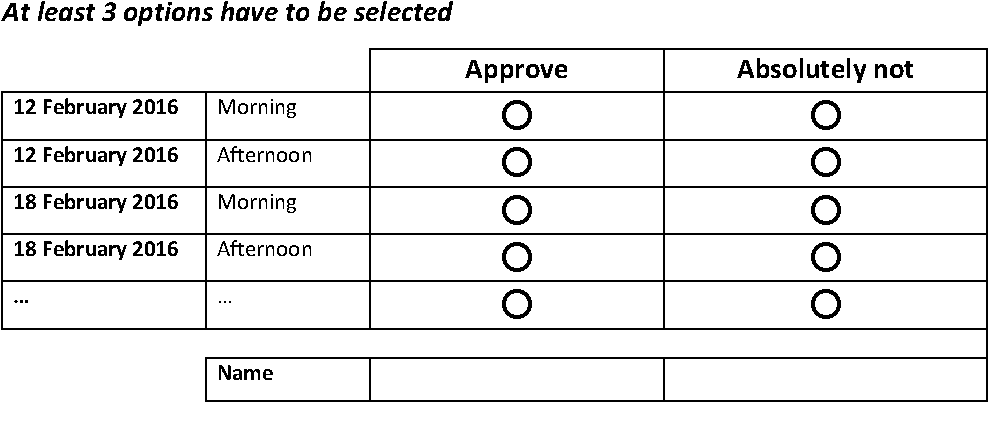
\includegraphics[width=.5\textwidth]{img/Voting.pdf}
\end{center}
%\end{parchment}

\begin{itemize}
\item No preference of any student should be weighted higher than another one's
\item Solution (exam schedule) is a shared decision

\end{itemize}
\end{frame}

\begin{frame}[fragile]{Exam Scheduling: Core Model}
See \texttt{exam-scheduling-approval.mzn}:
\begin{lstlisting}
% Exam scheduling example with just a set of 
% approved dates and *impossible* ones
include "globals.mzn";
include "soft_constraints/soft_constraints.mzn";

int: n; set of int: STUDENT = 1..n; 
int: m; set of int: DATE = 1..m;
array[STUDENT] of set of DATE: possibles;
array[STUDENT] of set of DATE: impossibles;

% the actual decisions
array[STUDENT] of var DATE: scheduled;

int: minPerSlot = 0; int: maxPerSlot = 4;
constraint global_cardinality_low_up(scheduled % minPerSlot, maxPerSlot
constraint forall(s in STUDENT) (not (scheduled[s] in impossibles[s])); 
 
\end{lstlisting}
\end{frame}

\begin{frame}[fragile]{Exam Scheduling: Preferences}
See \texttt{exam-scheduling-approval.mzn}:
\begin{lstlisting}
% have a soft constraint for every student
nScs = n;
penalties = [ 1 | n in STUDENT]; % equally important in this case 

constraint forall(s in STUDENT) ( 
     (scheduled[s] in possibles[s]) <-> satisfied[s] ) ;
var DATE: scheduledDates;
% constrains that "scheduledDates" different 
% values (appointments) appear in "scheduled"
constraint  nvalue(scheduledDates, scheduled);

% search variants 
solve 
:: int_search(satisfied, input_order, indomain_max, complete)
search minimize_lex([scheduledDates, violateds]);   % pro teachers
%search minimize_lex([violateds, scheduledDates]); % pro students
\end{lstlisting}
\end{frame}


\begin{frame}[fragile]{Exam Scheduling: Real Instance}

\begin{itemize}
\item Collected preferences of 33 students
\item over 12 possible dates (6 days, morning and afternoon)
\begin{itemize}
\item[-] \emph{Approval} set 
\item[-] \emph{Impossible} set 
\end{itemize}

\vspace*{2ex}

\item Aggregated via \alert{approval voting} (has nice voting-theoretical properties!)
\item At most 4 per appointment

\item Immediately (61 msec) found an optimal solution that
\begin{itemize}
\item[-] Is approved by \emph{every} student
\item[-] Is achieved with the minimal number of 9 dates 
\end{itemize}
\item Used Strategy:
\end{itemize}
\begin{lstlisting}
search minimize_lex([violateds, scheduledDates]); % pro students
\end{lstlisting}
\end{frame}

\begin{frame}[fragile]{Power Plant Scheduling}
\textbf{Goal}: Schedule plants such that they meet the \alert{demand}; See \texttt{unitCommitment.mzn}

\tikzset{
    trajectory/.style={issegrey},
    emph/.style={isseorange},
    trajectorynode/.style={issegrey},
    demand/.style={MidnightBlue, thick},
    firstTraj/.style={ForestGreen},
    secTraj/.style={BrickRed}
} 
\begin{figure}
\begin{tikzpicture}[scale=1.0]
    % Draw axes
    \draw [<->,thick] (0,5) node (yaxis) [above] {$P(t)$}
        |- (8.5,0) node (xaxis) [right] {$t$};
        
    \node[overlay,text width=1.9cm, text centered, anchor=south, right] at (7.7,4.5)
    { \small 
    \begin{itemize} 
    \item[] { \color{MidnightBlue} \onslide<2->{\textbf{Demand}} } 
    \item[] { \color{ForestGreen} \onslide<3->{Plant $a$} } 
    \item[] { \color{BrickRed} \onslide<4->{Plant $b$} }  
    \item[] { \color{isseorange} \onslide<5->{\textbf{Supply}} }    
    \end{itemize}
    };        
       
	
%	\node[text width = 1.5cm ,text centered, anchor=west, right] at (2.5, 1)
%	{
%		$\mathbf{+}$
%	};
	
    %\node[text width=2.5cm, text centered, anchor=west, right] at (4,-.5)
    %{
    %		Kraftwerk $\mathsf{b}$
	%}; 
	
	%\node[text width = 1.5cm ,text centered, anchor=west, right] at (6.5, 1)
	%{
	%	$\mathbf{=}$
%	};
	%\node[text width=2.5cm, text centered, anchor=west, right] at (8,-.5)
    %{
    %		Demand
	%};      
    
     % draw second trajectory first graph 
     \onslide<2->{
    \draw[trajectory,demand] (0,3.9) coordinate (d20) -- (1,4.6) coordinate (d21);
    \draw[trajectory,demand] (d21) -- (2,4.4) coordinate (d22);
    \draw[trajectory,demand] (d22) -- (3,4.7) coordinate (d23);
    \draw[trajectory,demand] (d23) -- (4,3.5) coordinate (d24);
    \draw[trajectory,demand] (d24) -- (5,3.5) coordinate (d25);
    \draw[trajectory,demand] (d25) -- (6,3.5) coordinate (d26);
    \draw[trajectory,demand] (d26) -- (7,4.0) coordinate (d27);
    \draw[trajectory,demand] (d27) -- (8,4.5) coordinate (d28);
    
    % now for the circles
    \fill[trajectorynode,demand] (d21) circle (1pt);
    \fill[trajectorynode,demand] (d22) circle (1pt);
    \fill[trajectorynode,demand] (d23) circle (1pt);
    \fill[trajectorynode,demand] (d24) circle (1pt);    
    \fill[trajectorynode,demand] (d25) circle (1pt);
    \fill[trajectorynode,demand] (d26) circle (1pt);
    \fill[trajectorynode,demand] (d27) circle (1pt);
    \fill[trajectorynode,demand] (d28) circle (1pt);
    }
        
    \onslide<3->{
    % now for the first plant   
    \draw[trajectory,firstTraj] (0,1.9) coordinate (p10) -- (1,2.0) coordinate (p11);
    \draw[trajectory,firstTraj] (p11) -- (2,2.4) coordinate (p12);
    \draw[trajectory,firstTraj] (p12) -- (3,2.4) coordinate (p13);
    \draw[trajectory,firstTraj] (p13) -- (4,2.2) coordinate (p14);
    \draw[trajectory,firstTraj] (p14) -- (5,2.4) coordinate (p15);
    \draw[trajectory,firstTraj] (p15) -- (6,2.4) coordinate (p16);
    \draw[trajectory,firstTraj] (p16) -- (7,2.4) coordinate (p17);                   
    \draw[trajectory,firstTraj] (p17) -- (8,2.6) coordinate (p18);
    
    	\onslide<6>{
       \draw[trajectory,firstTraj,very thick] (p11) -- (p12);	
       \node[overlay,align=left,rectangle callout,%
             callout absolute pointer=(p11.west),xshift=-.5cm,yshift=-1.5cm,fill=isseorange!50] at (p12) {
            \scriptsize \textbf{Must} ramp up \\ \scriptsize due to inertia};
       
	}    
    
 	\onslide<8>{
       \draw[trajectory,firstTraj,very thick] (p15) -- (p16);	
       \draw[trajectory,firstTraj,very thick] (p16) -- (p17);
       
          \node[overlay,align=left,rectangle callout,%
             callout absolute pointer=(p16.north),xshift=-.5cm,yshift=0.55cm,fill=isseorange!50] at (p15) {
           \scriptsize  Wait 2 steps for \\ \scriptsize further ramp-up};
	} 
	
    % now for the circles of the first graph
    \fill[trajectorynode,firstTraj] (p11) circle (1pt);
    \fill[trajectorynode,firstTraj] (p12) circle (1pt);
    \fill[trajectorynode,firstTraj] (p13) circle (1pt);
    \fill[trajectorynode,firstTraj] (p14) circle (1pt);    
    \fill[trajectorynode,firstTraj] (p15) circle (1pt);
    \fill[trajectorynode,firstTraj] (p16) circle (1pt);
    \fill[trajectorynode,firstTraj] (p17) circle (1pt);
    \fill[trajectorynode,firstTraj] (p18) circle (1pt);        
    }
    
    \onslide<4->{
    % now for the second plant   
    \draw[trajectory,secTraj] (0,2.0) coordinate (p20) -- (1,2.6) coordinate (p21);
    \draw[trajectory,secTraj] (p21) -- (2,2.0) coordinate (p22);
    \draw[trajectory,secTraj] (p22) -- (3,2.2) coordinate (p23);
    \draw[trajectory,secTraj] (p23) -- (4,1.5) coordinate (p24);
    \draw[trajectory,secTraj] (p24) -- (5,1.4) coordinate (p25);
    \draw[trajectory,secTraj] (p25) -- (6,1.2) coordinate (p26);
    \draw[trajectory,secTraj] (p26) -- (7,1.6) coordinate (p27);                   
    \draw[trajectory,secTraj] (p27) -- (8,1.9) coordinate (p28);
	\onslide<6>{
       \draw[trajectory,secTraj,very thick] (p21) -- (p22);	
       \node[overlay,align=left,rectangle callout,%
             callout absolute pointer=(p21.north),xshift=+1cm,yshift=.5cm,fill=isseorange!50] at (p21) {
            \scriptsize Has to compensate};
	}    
	
	\onslide<7>{
       \draw[trajectory,secTraj,very thick] (p23) -- (p24);	
       \node[overlay,align=left,rectangle callout,%
             callout absolute pointer=(p24.south),xshift=+1cm,yshift=-.8cm,fill=isseorange!50] at (p24) {
             \scriptsize Cannot ramp down further};
	}    
    
     % now for the circles of the second graph
    \fill[trajectorynode,secTraj] (p21) circle (1pt);
    \fill[trajectorynode,secTraj] (p22) circle (1pt);
    \fill[trajectorynode,secTraj] (p23) circle (1pt);
    \fill[trajectorynode,secTraj] (p24) circle (1pt);    
    \fill[trajectorynode,secTraj] (p25) circle (1pt);
    \fill[trajectorynode,secTraj] (p26) circle (1pt);
    \fill[trajectorynode,secTraj] (p27) circle (1pt);
    \fill[trajectorynode,secTraj] (p28) circle (1pt);
    }
    
    \onslide<5->{
    % draw joint production first graph 
    \draw[trajectory,emph] (0,3.9) coordinate (s20) -- (1,4.6) coordinate (s21);
    \draw[trajectory,emph] (s21) -- (2,4.4) coordinate (s22);
    \draw[trajectory,emph] (s22) -- (3,4.6) coordinate (s23);
    \draw[trajectory,emph] (s23) -- (4,3.7) coordinate (s24);
    \draw[trajectory,emph] (s24) -- (5,3.8) coordinate (s25);
    \draw[trajectory,emph] (s25) -- (6,3.6) coordinate (s26);
    \draw[trajectory,emph] (s26) -- (7,4.0) coordinate (s27);
    \draw[trajectory,emph] (s27) -- (8,4.5) coordinate (s28);
    
	% now for the circles of the sum
    \fill[trajectorynode,emph] (s21) circle (1pt);
    \fill[trajectorynode,emph] (s22) circle (1pt);
    \fill[trajectorynode,emph] (s23) circle (1pt);
    \fill[trajectorynode,emph] (s24) circle (1pt);    
    \fill[trajectorynode,emph] (s25) circle (1pt);
    \fill[trajectorynode,emph] (s26) circle (1pt);
    \fill[trajectorynode,emph] (s27) circle (1pt);
    \fill[trajectorynode,emph] (s28) circle (1pt);
    }
    
	\node[text centered, anchor=north] at (1,0) { 1 }; \draw[thick] (1,0.05) -- (1,-.05);
	\node[text centered, anchor=north] at (2,0) { 2 }; \draw[thick] (2,0.05) -- (2,-.05);
	\node[text centered, anchor=north] at (3,0) { 3 }; \draw[thick] (3,0.05) -- (3,-.05);	
	\node[text centered, anchor=north] at (4,0) { 4 }; \draw[thick] (4,0.05) -- (4,-.05);
	\node[text centered, anchor=north] at (5,0) { 5 }; \draw[thick] (5,0.05) -- (5,-.05);
	\node[text centered, anchor=north] at (6,0) { 6 }; \draw[thick] (6,0.05) -- (6,-.05);
	\node[text centered, anchor=north] at (7,0) { 7 }; \draw[thick] (7,0.05) -- (7,-.05);	
	\node[text centered, anchor=north] at (8,0) { 8 }; \draw[thick] (8,0.05) -- (8,-.05);
	    

\end{tikzpicture}
\end{figure}  
\end{frame}

\begin{frame}[fragile]{Power Plant Scheduling: Core Model}
\begin{lstlisting}
include "soft_constraints/soft_constraints_noset.mzn";
include "soft_constraints/cr_types.mzn";
include "soft_constraints/cr_weighting.mzn";
% ground penalties using the appropriate weighting
penalties = [weighting(s, SOFTCONSTRAINTS, crEdges, true) 
                 | s in SOFTCONSTRAINTS];

int: T = 5; set of int: WINDOW = 1..T;
array[WINDOW] of float: demand = [10.0, 11.3, 15.2, 20.7, 19.2];

int: P = 3; set of int: PLANTS = 1..P;
array[PLANTS] of float: pMin  = [12.0, 5.0, 7.3];
array[PLANTS] of float: pMax  = [15.0, 11.3, 9.7];

array[WINDOW, PLANTS] of var 0.0..15.0: supply; 
var float: obj;

constraint obj = sum(w in WINDOW) ( abs( sum(p in PLANTS) 
           (supply[w, p]) - demand[w] ) );

\end{lstlisting}
\end{frame}

\begin{frame}[fragile]{Power Plant Scheduling: Soft Constraints}
\begin{lstlisting}
% ground penalties using the appropriate weighting
penalties = [weighting(s, SOFTCONSTRAINTS, crEdges, true) 
                 | s in SOFTCONSTRAINTS];
[...]

% some soft constraints
constraint supply[1, 2] >= 6.0 <-> satisfied[1]; 
constraint supply[2, 2] >= 6.0 <-> satisfied[2]; 


% constraint time step 1 seems more urgent
nCrEdges = 1;
crEdges = [| 2, 1 |];

% could do something more sophisticated here
solve minimize obj + penSum;
\end{lstlisting}
$\rightarrow$ Library works with MIP (\emph{Mixed Integer Programming}) as well!
\end{frame}



\begin{frame}[fragile]{Switching PVS Type}
Concrete PVS are instantiated by importing the appropriate \texttt{pvs\_x.mzn} file.
\lstinputlisting{models/m1.mzn}
\end{frame}

\begin{frame}[fragile]{Consistency Checks}
Vital, when designing constraint relationships: \alert{avoid cycles!}

\texttt{model-inconsistent.mzn}
\lstinputlisting{models/model-inconsistent.mzn}
\end{frame}

\begin{frame}[fragile]{Consistency Checks}
\begin{center}

\includegraphics[width=.7\textwidth]{img/errorMz.png}
\end{center}
Better: Add model checks to detect cyclic relationships!
\end{frame}

\begin{frame}[fragile]{Consistency Checks: Assertions}
\texttt{model-inconsistent-safe.mzn}
\lstinputlisting{models/model-inconsistent-safe.mzn}
\end{frame}

\begin{frame}[fragile]{Consistency Checks: Assertions}
\texttt{minisearch model-inconsistent-safe.mzn}

\vspace*{2ex}

\begin{verbatim}
minizinc/std/soft_constraints/cr_consistency.mzn:46:
  in call 'assert'
  Assertion failed: Relationship is cyclic!

\end{verbatim}

\end{frame}

\begin{frame}[fragile]{Transitive Closure}
\vspace*{2ex}

For larger constraint relationships, it can be more convenient 
to just specify a directed acyclic graph and have the closure (all transitive edges)
be calculated automatically.

\centering
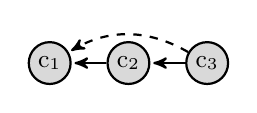
\begin{tikzpicture}[auto,
                    ->,>=stealth',shorten >=1pt,thick,
                    node distance=.7cm,inner sep=2pt,
                    constraint/.style={circle,fill=black!15,draw,font=\sffamily\small}]
\node[constraint node] (1) at (0, 0)                   {$\mathrm{c}_1$};
\node[constraint node] (2) at ($ (1) + (1, 0) $) {$\mathrm{c}_2$};  
\node[constraint node] (3) at ($ (1) + ( 2, 0) $) {$\mathrm{c}_3$};  
%  
\path[every node/.style={font=\sffamily\tiny}]
  (2) edge (1)
  (3) edge (2)
  (3) edge[dashed,bend right] (1)
  ;
\end{tikzpicture}
\lstinputlisting{models/cr_trans_example.mzn}
\end{frame}

\begin{frame}[fragile]{Variable Ordering}
Recall that \texttt{soft\_constraints.mzn} defines a variable ordering with 
weights in descending order:

\vspace*{1ex}

\begin{lstlisting}
% find the sorted permutation of soft constraint instances
array[SOFTCONSTRAINTS] of SOFTCONSTRAINTS: sortPermScs = 
    arg_sort(penalties);
% invert, since arg_sort use <= and we need decreasing order
array[SOFTCONSTRAINTS] of SOFTCONSTRAINTS: mostImpFirst = 
    [ sortPermScs[nScs-s+1] | s in SOFTCONSTRAINTS]; 

\end{lstlisting}

\vspace*{1ex}

We can use this ordering to try out important constraints early on in search.
\end{frame}

\begin{frame}[fragile]{Variable Ordering: Demo}
\texttt{smallexample.mzn}:

\lstinputlisting{models/smallexample.mzn}
\small 
\begin{verbatim}
Obj: 4 by x=1, y=1,z=1
----------
Obj: 3 by x=1, y=1,z=3
----------
Obj: 1 by x=1, y=2,z=1
----------
==========
\end{verbatim}
\end{frame}

\begin{frame}[fragile]{Variable Ordering: Demo}
\texttt{smallexample-mif.mzn}:

\lstinputlisting{models/smallexample-mif.mzn}
\small 
\begin{verbatim}
Obj: 1 by x=1, y=2,z=1
----------
==========
\end{verbatim}
(finds the optimal solution at first try)
\end{frame}

\begin{frame}[allowframebreaks]
        \frametitle{References}
        \bibliographystyle{apalike}
        \bibliography{../common.bib}
\end{frame}


\end{document}

